% Page settings
\documentclass[notitlepage,12pt]{article}
\usepackage{fancyvrb, verbatim, listings}                                  % Various for inserting/hosting code
\usepackage[nodisplayskipstretch]{setspace} \setstretch{1.5}               % Space between lines (customisable)
\usepackage[margin=2.54cm]{geometry}                                       % Set margins (standard is 2.54cm)
\usepackage[UKenglish,cleanlook]{isodate}                                  % Set default date and date display
\usepackage{fancyhdr} \pagestyle{fancy}                                    % Line the top of the page
\usepackage[activate={true,nocompatibility},final,tracking=true,kerning=true,spacing=true,factor=1100,stretch=10,shrink=10]{microtype}
\microtypecontext{spacing=nonfrench}                                       % Change font and minor spacings to look nicer
%% Packages to use:
% Tables + figures
\usepackage{graphicx}                                                      % control over the import of graphics
\usepackage[table,dvipsnames]{xcolor}                                      % Define tables (with colour control)
\usepackage{float}                                                         % Control over graphics + tables float
\usepackage[justify]{ragged2e}                                             % control over text alignment
\usepackage{booktabs}                                                      % caption graphics + tables (with name in bold)
\usepackage[labelfont=bf]{caption} 
\usepackage{subcaption}
\usepackage[shortlabels]{enumitem} \setlist[enumerate]{leftmargin=0pt}     % Customisable lists
% caption graphics + tables (with name in bold)
\usepackage{tikz}
\usetikzlibrary{shapes,decorations,decorations.pathreplacing,arrows,calc,arrows.meta,fit,positioning}
\tikzset{
    auto,node distance =1 cm and 1 cm,semithick,
    state/.style ={ellipse, draw, minimum width = 0.7 cm},
    point/.style = {circle, draw, inner sep=0.04cm,fill,node contents={}},
    bidirected/.style={Latex-Latex,dashed},
    el/.style = {inner sep=2pt, align=left, sloped}
}
%\usepackage{pgfplots} \pgfplotsset{compat=1.16}                            % Automatic graphing, read https://www.overleaf.com/learn/latex/pgfplots_package for examples
% Maths + numbers
\usepackage{mathtools}                                                     % Various maths functions
\usepackage{amssymb}                                                       % Various maths functions
\usepackage{amsmath}                                                       % Various maths functions
\usepackage{dsfont}                                                        % Various maths functions
\usepackage{centernot}                                                     % center \not usage
\usepackage{siunitx} \sisetup{round-mode=places, round-precision=3}        % Formalise use of units and numbers among text
\usepackage{amsthm}                                                        % NEvrionemtn for theorems.
\newtheorem{theorem}{Theorem}                                              % Define theorem environment.
\newtheorem{assumption}{Assumption}                                        % Define assumptions environment ahead of theorems.
\newtheorem{definition}{Definition}                                        % Define definitions environment ahead of theorems.
\DeclareMathOperator{\eps}{\varepsilon}                                    % epsilon short hand shortcut
\DeclareMathOperator{\st}{\text{ s.t. }}                                   % "such that" short hand shortcut
\DeclareMathOperator{\then}{\text{ then }}                                 % "then" in equation shortcut
\DeclareMathOperator{\ifeq}{\text{ if }}                                   % "if" in equation shortcut
\DeclareMathOperator{\oreq}{\text{ or }}                                   % "or" in equation shortcut
\DeclareMathOperator{\andeq}{\text{ and }}                                 % "and" in equation shortcut
\DeclareMathOperator{\all}{,\; \text{ for }}                                    % all (with spacing) in equation shortcut
\DeclareMathOperator{\N}{\mathbb{N}}                                       % N, natural number, shortcut
\DeclareMathOperator{\R}{\mathbb{R}}                                       % R, real number, shortcut
\DeclareMathOperator{\Ll}{\mathcal{L}}                                     % L, Lagrangian, shortcut
\renewcommand{\vec}[1]{\boldsymbol{\mathit{#1}}}                           % vector notation shortcut
\newcommand{\mat}[1]{\boldsymbol{\mathit{#1}}}                             % matrix notation shortcut
\DeclarePairedDelimiter\abs{\lvert}{\rvert}                                % absolute value notation shortcut
\DeclarePairedDelimiter\norm{\lVert}{\rVert}                               % norm notation shortcut
\newcommand{\Prob}[1]{\Pr\left( #1 \right)}                         % SHortcut for probability notation
\newcommand{\Probgiven}[2]{\Pr\left( #1 \, \middle\vert \, #2 \right)} % SHortcut for probability notation, given
\newcommand{\E}[2][]{\mathbb{E}_{#1} \left[ #2 \right]}                    % Expectation (with optional subscript) shortcut
\newcommand{\Egiven}[3][]{\mathbb{E}_{#1} \left[ #2 \, \middle\vert \, #3 \right]} % Expectation given (with optional subscript) shortcut
\newcommand{\Var}[2][]{\text{Var}_{#1} \left( #2 \right)}                  % Variation (with optional subscript) shortcut
\newcommand{\Cov}[1]{\text{Cov} \left( #1 \right)}                         % Covariance (with optional subscript) shortcut
\newcommand{\median}[1]{\text{median} \left( #1 \right)}                   % Median (with optional subscript) shortcut
\newcommand{\indicator}[1]{\mathds{1}\left\{ #1 \right\}}                  % SHortcut for indicator function
\newcommand{\diff}[2][]{\frac{d#1}{d#2}}                                   % SHortcut for differential fraction as a function
\newcommand{\partialdiff}[2][]{\frac{\partial#1}{\partial#2}}              % SHortcut for partial differential fraction as a function
\newcommand{\converge}[1]{\xrightarrow{ #1 \to\infty}}                     % SHortcut for convergence arrow
\renewcommand{\hat}[1]{\widehat{#1}}                                       % Default estimator notation is widehat
\renewcommand{\bar}[1]{\overline{#1}}                                      % Make over bar look nicer
\renewcommand{\tilde}[1]{\widetilde{#1}}                                   % Make over tilde look better
\newcommand{\indep}{\, \raisebox{0.05em}{\rotatebox[origin=c]{90}{$\models$}} \,}% Statistical independence symbol.
\definecolor{ao(english)}{rgb}{0.0, 0.5, 0.0}                              % Define dark green colour 
% Citations
\usepackage[longnamesfirst]{natbib}                                        % Citation package, see https://en.wikibooks.org/wiki/LaTeX/Bibliography_Management#Natbib
\usepackage[backref=page]{hyperref}                                        % Allow for links across the text, with colour options
\hypersetup{colorlinks=true, linkcolor=blue, citecolor=blue, filecolor=magenta, urlcolor=blue}
\def\sectionautorefname~#1\null{Section~#1\null}                           % Fix autoref for sections
\def\subsectionautorefname~#1\null{Subsection~#1\null}                     % Fix autoref for subsections
\def\subsubsectionautorefname~#1\null{Subsubsection~#1\null}               % Fix autoref for subsubsections
\def\equationautorefname~#1\null{Equation~(#1)\null}                       % Fix autoref for equations
% IMPORTANT: follow style guide here https://github.com/Wookai/paper-tips-and-tricks


%%%%%%%%%%%%%%%%%%%%%%%%%%%%%%%%%%%%%%%%
%% Title page
% Author
\singlespacing
\author{Senan Hogan-Hennessy\thanks{
    % This work has been supported by research funding from the Economics Department, Cornell University.
    For helpful comments I thank
    Lexin Cai,
    Neil Cholli,
    Hyewon Kim,
    Jiwoo Kim,
    Bart de Koning,
    Luk\'a\u{s} Laff\'ers,
    Jiwon Lee,
    Yiqi Liu,
    Douglas Miller,
    Zhuan Pei,
    Brenda Prallon,
    Evan Riehl,
    and
    Yiwei Sun.
    Some preliminary results previously circulated in an earlier version of the working paper ``The Direct and Indirect Effects of Genetics and Education.''
    I thank seminar participants at Cornell University (2025)
    %and the Econometrics World Congress (2025)
    for helpful discussion.
    Any comments or suggestions may be sent to me at \href{mailto:seh325@cornell.edu}{\nolinkurl{seh325@cornell.edu}}, or raised as an issue on the Github project.
    } \\
    \vspace{0.1cm}
    Economics Department, Cornell University\footnote{
        Address: Uris Hall \#447, Economics Department, Cornell University NY 14853 USA.
    }
}
% Title
\title{Causal Mediation in Natural Experiments}
\date{
    First draft: 12 February 2025 \\
    This version:
    \today \\ \vspace{0.25cm}
    \textbf{\textit{Work in Progress,
    newest version
    \href{https://github.com/shoganhennessy/mediation-natural-experiment/blob/main/mediation-natural-experiment-2025.pdf}{available here}.}}
    \vspace{-1.0cm}
}
\rhead{\today}
\lhead{Causal Mediation in Natural Experiments.}
% Begin
\begin{document}
\clearpage
\maketitle
\thispagestyle{empty}
% Abstract
\begin{abstract}
    \noindent
Natural experiments are a cornerstone of applied economics, providing settings for estimating causal effects with a compelling argument for treatment ignorability.
Economists are often interested in understanding the mechanisms through which causal treatment effects operate, and Causal Mediation (CM) methods aid this by estimating how much of the treatment effect operates through a proposed mediator.
The most popular CM approach relies on assumptions which are unrealistic in natural experiment settings: assuming the mediator is conditionally ignorable --- in addition to the ignorability argument for the initial treatment.
This paper shows that this approach leads to biased inference, solving for explicit bias terms when the mediator is not ignorable.
Using the case of a Roy model for a mediator, I show that individuals' selection based on expected gains and costs is inconsistent with mediator ignorability without implausible behavioural assumptions, and that bias terms are large in practice.
I show a control function approach, which overcomes these hurdles if monotonicity holds, using cost of mediator take-up as an instrument.
Simulations confirm that this method corrects for persistent bias in conventional CM estimates, and performs comparably to a selection-on-observables approach when the structural assumptions do not hold.
% I illustrate the approach by estimating the proportion of the causal effect of genes associated with education that operates via a direct genetic channel versus indirectly through extended schooling.
% Finally, I provide an implementation of this method in the \textit{R} package \textit{mediate-controlfun}, offering an accessible tool for robust mediation analysis in natural experiment settings.
This approach gives applied researchers a practical method to estimate CM effects when they can only establish a credible argument for randomisation of the initial treatment, as is common in natural experiments.

\vspace{0.5cm}
\noindent
\textbf{Keywords:}
Direct/indirect effects, quasi-experiment, selection, control function.

\vspace{0.1cm}
\noindent
\textbf{JEL Codes:}
D31, D91, I24, J24, Z00.

\end{abstract}

%%%%%%%%%%%%%%%%%%%%%%%%%%%%%%%%%%%%%%%%%
%% Starting the paper
\newpage
\setcounter{page}{1}
\doublespacing
% Introduction section
\noindent
%\section{Introduction}
%\label{sec:intro}
% \textbf{The introduction formula \url{https://blogs.ubc.ca/khead/research/research-advice/formula}.}
%\textbf{Hook:}
Economists use natural experiments to credibly answer social questions, when an experiment was infeasible.
For example, does access to health insurance causally improve health and well-being \citep{finkelstein2008oregon}?
Natural experiments are settings which answer these questions, but give little indication of how these effects came about.
Causal Mediation (CM) aims to estimate the mechanisms behind causal effects, by estimating how much of the treatment effect operates through a proposed mediator.
For example, do causal gains from access to health insurance come mostly from starting to utilise healthcare more often, or are there other direct effects?
This study of mechanisms behind causal effects broadens the economic understanding of social settings studied with natural experiments.
This paper shows that the conventional approach to estimating CM effects is inappropriate in a natural experiment setting, provides a theoretical framework for how bias operates, and develops an approach to correctly estimate CM effects under alternative assumptions.
These methods contrast the current practice in applied economics of providing suggestive evidence of mechanisms, which does not identify or quantify causal effects.

% Paragraph here: how do applied economists currently do it?
% Summarise my work with the Finkelstein+ data.

%\textbf{Question:}
This paper starts by considering conventional CM methods in a natural experiment setting.
Conventional CM methods rely on assuming the initial treatment, and the subsequent mediator, are both ignorable \citep{imai2010identification}.
In a natural experiment setting, however, this may not hold true; 
winners of the Oregon Health Insurance Experiment wait-list lottery randomly received access to health insurance, but then chose of their own free will how often to use healthcare.
Here, conventional CM estimates for the average direct and indirect effects will be contaminated by bias terms, from not accounting for selection-into-healthcare.
Indeed, it is unlikely conventional CM estimates in any natural experiment will lead to credible causal effects, unless researchers use another natural experiment to isolate random variation in the mediator (at the same time as using one for the initial treatment).

I consider an alternative approach to estimating CM effects, adjusting for unobserved selection-into-mediator via identifying the marginal treatment effect of the mediator.
This solves the identification problem with structural assumptions for selection-into-mediator --- mediator monotonicity and selection based on benefits --- and requires a valid cost instrument for mediator take-up.
While these assumptions are strong, they are plausible in many applied settings.
Mediator monotonicity aligns with conventional theories for selection-into-treatment, and is accepted widely in many applications using an instrumental variables research design.
Selection based on costs and benefits is central to economic theory, and is the dominant concern for judging empirical designs that identify causal effects.
Access to valid instrumental variation is a strong condition, though is important to avoid further modelling assumptions; the most compelling example is using variation in mediator take-up costs as an instrument.
This approach is not perfect in every setting: the structural assumptions are strong, and are tailored to selection-into-mediator concerns pertinent to economic applications.
Indeed, this approach provides no safe harbour for estimating CM effects if these structural assumptions do not hold true.

%Paragraph on the results of the Oregon experiment.

%\textbf{Antecedents:}
Assuming the mediator is quasi-randomly assigned conveniently ignores selection by assuming either (1) people na\"ively made decisions to take or refuse a mediator, or (2) a researcher controlled for everything relevant to this decision.
This assumption might be reasonable when studying single-celled organisms in a laboratory --- their ``decisions'' are simple and mechanical.
Social scientists, however, study humans who make complex choices based on costs, benefits, and preferences --- which are only partially observed by researchers, at best.
Assuming a mediator is ignorable in social science contexts is often unrealistic.
In practice, the main setting where mediator ignorability becomes credible is when researchers find another natural experiment affecting the mediator --- a rare occurrence given how difficult it is to find one source of random variation for a treatment, let alone another independent source for a mediator, at the same time.

The applied economics literature has been hesitant to use explicit CM methods, instead providing suggestive evidence for mechanisms,\footnote{
    See \cite{blackwell2024assumption} for an overview of this approach, from the empirical politics literature.
} sometimes accompanied by a practice of controlling for a proposed mediator.
Neither of these approaches have a causal interpretation.
A new strand of the econometric literature has developed estimators for explicit CM analyses under a variety of strategies.
These include overlapping quasi-experimental research designs \citep{deuchert2019direct,frolich2017direct}, functional form restrictions \citep{heckman2015econometric,heckman2013understanding}, partial identification \citep{flores2009identification}, or a hypothesis test of full mediation through observed channels \citep{kwon2024testing} --- see \cite{huber2019review} for an overview.\footnote{
    An alternative method to estimate CM effects is ensuring treatment and mediator ignorability holds by a running two randomised controlled trials for both treatment and mediator, at the same time.
    This set-up has been considered in the literature previously, in theory \citep{imai2013experimental} and in practice \citep{ludwig2011mechanism}.
}
The new literature has arisen in implicit acknowledgement that suggestive evidence of mechanisms, or a conventional approach to CM, can lead to biased inference and needs alternative methods for credible inference.

%\textbf{Value-added:}
I develop a framework showing exactly how selection bias contaminates CM estimates when mediator choices are driven by unobserved gains --- settings where none of the natural experiment research designs in the previously cited papers apply (i.e., the mediator is not ignorable).
This provides a rigorous warning to applied economists against uncritically applying conventional CM methods to investigate mechanisms in natural experiments --- as is common in the applied fields of epidemiology, psychology, and medicine.
Selection based on costs and benefits, as in the \cite{roy1951some} model, is at odds with assuming a mediator is randomly assigned in an observational setting, so I import methods grounded in labour economic theory to solve the identification problem.

Identifying CM effects via the marginal treatment effect of the mediator requires mediator take-up respond only positively to the initial treatment (monotonicity), which implies mediator selection follows a selection model.
Second, it assumes that mediator take-up is motivated by mediator benefits.
Last, it requires a valid instrument for mediator take-up, to avoid relying on parametric assumptions on unobserved selection.
This approach to identifying CM effects imports insights from the instrumental variables literature, connecting the influential \cite{imai2010identification} approach to CM with the economics literature on selection-into-treatment and marginal treatment effects \citep{vytlacil2002independence,heckman2004using,heckman2005structural,florens2008identification,kline2019heckits}.
%\footnote{
%    Indeed, this paper does not invent control function methods, instead noting their applicability in this setting.
%    See \cite{wooldridge2015control,imbens2007nonadditive} for general overviews of the approach.
%}
\cite{frolich2017direct} have previously explored identification of CM effects with a control function in the context of two instruments (one each for treatment and mediator) and a continuous mediator.
This paper considers the marginal treatment effect of a binary mediator, with a correspondingly different identification analysis and resulting estimation strategies.

%\textbf{Road-map:}
This paper proceeds as follows.
\autoref{sec:lottery} describes the dominant approach in economics for studying mechanisms behind treatment effects, illustrating with data from the Oregon Health Insurance Experiment.
% and surveys economic research.
\autoref{sec:mediation} introduces the formal framework for CM, and develops expressions for bias in CM estimates in natural experiments.
\autoref{sec:applied} describes this bias in applied settings with (1) a regression framework, (2) a setting with selection based on costs and benefits.
\autoref{sec:selectionmodel} purges bias from CM estimates by identifying CM effects via the marginal treatment effect of the mediator, with a control function adjustment.
\autoref{sec:controlfun} demonstrates how to estimate CM effects with this approach, with either parametric or semi-parametric methods, giving supporting simulation evidence.
\autoref{sec:oregon} returns to the Oregon Health Insurance Experiment, providing credible estimates of access to health insurance effects on self-reported health and well-being mediated through healthcare usage.
\autoref{sec:conclusion} concludes.

% Design-based Framework
\section{Direct and Indirect Effects}
\label{sec:mediation}
Causal mediation decomposes causal effects into two channels, through a mediator (indirect effect) and through all other paths (direct effect).
To develop notation for direct and indirect effects, write $Z_i$ for an exogenous binary treatment, $D_i$ a binary mediator, and $Y_i$ an outcome for individuals $i = 1, \hdots, n$.\footnote{
    Other literatures use different notation.
    For example, \cite{imai2010identification} write $T_i, M_i, Y_i$ for the randomised treatment, mediator, and outcome, respectively.
    I use $Z_i, D_i, Y_i$ to stick to the instrumental variables notation \cite{angrist1996identification}, more familiar in empirical economics \citep{angrist2009mostly}. 
}
The outcomes are a sum of their potential outcomes.\footnote{
    This paper exclusively focuses on the binary case.
    See \cite{huber2020direct} for a discussion of CM with continuous treatment and/or mediator, and the assumptions required.
}
\begin{align*}
    D_i &= Z_i       D_i(1)
        + (1 - Z_i) D_i(0),  \\
    Y_i &= Z_i       Y_i(1, D_i(1))
        + (1 - Z_i) Y_i(0, D_i(0)).
\end{align*}

%Write $\vec X_i$ for a set of control variables, and assume $Z_i$ is ignorable --- possibly conditional on $\vec X_i$.
Assume $Z_i$ is ignorable.\footnote{
    This assumption can hold conditional on covariates.
    To simplify notation in this section, leave the conditional part unsaid, as it changes no part of the identification framework.
}
\[ Z_i \indep  D_i(z), Y_i(z', d), \textnormal{ for } z, z', d = 0, 1 \]

There are only two average effects which are identified (without additional assumptions).
\begin{enumerate}
    \item The average first-stage refers to the effect of the treatment on mediator, $Z \to D$.
    \[ \Egiven{D_i}{Z_i = 1} - \Egiven{D_i}{Z_i = 0}
        = \E{D_i(1) - D_i(0)} \]
    It common in the economics literature to assume that $Z$ influences $D$ in at most one direction, $\Prob{D_i(1) \geq D_i(0)} = 1$ --- monotonicity \citep{imbens1994identification}.
    I assume monotonicity (and its conditional variant) holds through-out to simplify notation.\footnote{
        Assuming monotonicity also brings closer to the IV notation, and has other beneficial implications in this setting (see \autoref{sec:controlfun}).
    }
    \item The reduced-form effect refers to the effect of the treatment on outcome, $Z \to Y$, and is also known as the intent-to-treat effect in experimental settings, or total effect in causal mediation literature.
    \[ \Egiven{Y_i}{Z_i = 1} - \Egiven{Y_i}{Z_i = 0}
        = \E{Y_i(1, D_i(1)) - Y_i(0, D_i(0))} \]
\end{enumerate}
In this setting, $Z_i$ affects outcome $Y_i$ directly, and indirectly via the $D_i(Z_i)$ channel, with no reverse causality.
% The framework is general to any (conditionally) randomly assigned $Z_i$, intermiedate mediator $D_i$, and outcome $Y_i$.
%This section focuses on binary $Z_i, D_i = 0,1$, and not the continuous versions, to simplify the causal framework.%\footnote{
    %\autoref{appendix:continuous} relates the causal framework to continuous $Z_i,D_i$, which has little conceptual differences.}
On the other hand, mediation aims to decompose the reduced form effect of $Z \to Y$ into these two separate pathways.
\autoref{fig:scm-model} visualises the design, where the direction arrows denote the causal direction (and no reverse causality).
\begin{align*}
    \text{Average Indirect Effect (AIE), } D(Z) \to Y: \;\;\;&
        \E{Y_i(Z_i, D_i(1)) - Y_i(Z_i, D_i(0))} \\
    \text{Average Direct Effect (ADE), } Z \to Y: \;\;\;&
        \E{Y_i(1, D_i(Z_i)) - Y_i(0, D_i(Z_i))}
\end{align*}
Estimating the AIE answers the following question: how much of the causal effect $Z \to Y$ goes through the $D$ channel?
In an applied example, this could be how much does the effect of (random) military conscription goes through military service?
In an instrumental variables application, this direct effect is assumed to be zero for everyone (i.e., the exclusion restriction).
CM is a different framework attempting to explicitly model the direct effect, not assuming the ADE is zero.
Estimating the ADE answers the following equation: how much is left over after accounting for the $D$ channel?\footnote{
    In a non-parametric setting it is not necessary that the ADE and AIE sum to the total effect.
    See \cite{imai2010identification} for this point in full.
}
These CM effects are not separately identified without further assumptions.

\begin{figure}[h!]
    \centering
    \singlespacing
    \caption{Structural Causal Model for Causal Mediation.}
    \label{fig:scm-model}
    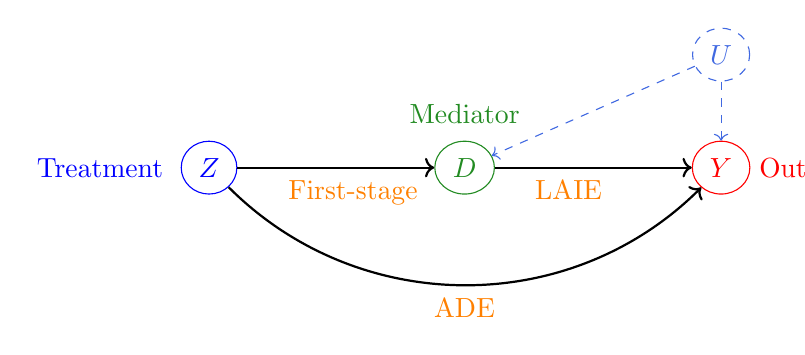
\begin{tikzpicture}
        \node[state,ForestGreen] (treatment) at (0,0) {$D$};
        \node[state,blue] (instrument) [left=2.5cm of treatment] {$Z$};
        \node[state,red] (outcome) [right=2.5cm of treatment] {$Y$};
        % Label Z, D, Y
        \node[color=ForestGreen] [above=0.1cm of treatment] (mediator) {Mediator};
        \node[color=blue] [left=0.1cm of instrument] {Treatment};
        \node[text width=0.1cm, color=red] [right=-0.01cm of outcome] {Outcome};
        % Draw the causal arrows
        \path[->, thick] (instrument) edge (treatment);
        \path[->, thick] (treatment) edge (outcome);
        \path[->, thick] (instrument) edge[bend right=45] (outcome);
        % Label direct and indirect effect
        \node[color=orange] [below left=-0.2cm and 0.2cm of treatment] {First-stage};
        \node[color=orange] [below right=-0.2cm and 0.5cm of treatment] {LAIE};
        \node[color=orange] [below=1.2cm of treatment] {ADE};
        % Add in the confounders
        %\node[state,RoyalPurple] (confounderX) [above=1.5cm of treatment] {$\vec{X}$};
        %\path[->,RoyalPurple] (confounderX) edge (treatment);
        %\node[color=RoyalPurple] [left=0.1cm of confounderX] {Observed controls};
        \node[state,dashed,RoyalBlue] (confounderU) [above=0.75cm of outcome] {$U$};
        \path[->,dashed,color=RoyalBlue] (confounderU) edge (treatment);
        \path[->,dashed,color=RoyalBlue] (confounderU) edge (outcome);
        %\node[color=RoyalBlue] [right=0.1cm of confounderU] {Unobserved confounder};
    \end{tikzpicture}
    \justify
    \footnotesize
    \textbf{Note}:
    This figures shows the structural causal model behind causal mediation.
    LAIE refers to the AIE (i.e., effect of the mediator $D \to Y$) local to $Z$ compliers, so that AIE $=$ average first-stage $\times$ LAIE.
    Unobserved confounder $U$ represents this paper's focus on the case that $D_i$ is not ignorable, by showing an implied unobserved confounder.
    \autoref{sec:regression} formally defines $U$ in this set-up.
\end{figure}

\subsection{Identifying Causal Mediation (CM) Effects}
The conventional approach to estimating direct and indirect effects assumes both $Z_i$ and $D_i$ are ignorable, conditional on a set of control variables $\vec X_i$.
\begin{definition}
    \label{dfn:seq-ign}
    Sequential Ignorability \citep{imai2010identification}.
    \begin{align}
        \label{eqn:seq-ign-Z}
        Z_i \indep  D_i(z), Y_i(z', d) \;\; &| \;\; \vec X_i,
            &\textnormal{ for } z, z', d = 0, 1 \\
        \label{eqn:seq-ign-D}
        D_i \indep Y_i(z', d) \;\; &| \;\; \vec X_i, Z_i = z', 
            &\textnormal{ for } z', d = 0, 1
    \end{align}
\end{definition}
Sequential ignorability assumes that the initial treatment $Z_i$ is assigned randomly, conditional on $\vec X_i$.
It then also assumes that, after $Z_i$ is assigned, that $D_i$ is assigned randomly conditional $\vec X_i, Z_i$.
If sequential ignorability, \ref{dfn:seq-ign}\eqref{eqn:seq-ign-Z} and \ref{dfn:seq-ign}\eqref{eqn:seq-ign-D}, holds then the ADE and AIE are identified by two-stage mean differences, after conditioning on $\vec X_i$.\footnote{
    \cite{imai2010identification} show a general identification statement; I show identification in terms of two-stage regression, notation for which is more familiar in economics.
    This reasoning is in line with G-computation reasoning \citep{robins1986g};
    \autoref{appendix:identification} states the \cite{imai2010identification} identification result, and then develops the two-stage regression notation which holds as a consequence of sequential ignorability.
}

\makebox[\textwidth]{\parbox{1.25\textwidth}{
\[ \E[D_i = d', \vec X_i]{
    \underbrace{\Egiven{Y_i}{Z_i = 1, D_i = d', \vec X_i} - \Egiven{Y_i}{Z_i = 0, D_i = d', \vec X_i}}_{\text{Second-stage regression, $Y_i$ on $Z_i$ holding $D_i$ constant}}}
    = \underbrace{\E{Y_i(1, D_i(Z_i)) - Y_i(0, D_i(Z_i))}}_{\text{Average Direct Effect (ADE)}} \]
\[ \E[Z_i = z', \vec X_i]{ \underbrace{\Big(
    \Egiven{D_i}{Z_i = 1, \vec X_i} - \Egiven{D_i}{Z_i = 0, \vec X_i} \Big)}_{\text{First-stage regression, $D_i$ on $Z_i$}}
    \times \underbrace{\Big(
    \Egiven{Y_i}{Z_i = z', D_i = 1, \vec X_i} - \Egiven{Y_i}{Z_i = z', D_i = 0, \vec X_i} \Big)}_{\text{Second-stage regression, $Y_i$ on $D_i$ holding $Z_i$ constant}} } \]
\[ = \underbrace{\E{Y_i(Z_i, D_i(1)) - Y_i(Z_i, D_i(0))}}_{\text{Average Indirect Effect (AIE)}} \]
}}
I refer to the estimands on the left-hand side as Causal Mediation (CM) estimands.
These estimands are typically estimated with linear models, with resulting estimates composed from OLS estimates \citep{imai2010identification}.
%\begin{align*}
%    D_i &= \phi + \pi Z_i
%        + \vec \psi_1' \vec X_i+ \eta_i \\
%    Y_i &= \alpha + \beta D_i + \gamma Z_i + \delta Z_i D_i
%        + \vec \psi_2' \vec X_i + \varepsilon_i
%\end{align*}
%And so the CM estimands are composed from OLS estimates,
%$\hat \gamma + \hat\delta \E{D_i}$ for the Average Direct Effect (ADE) and
%$\hat\pi \left(\hat \beta + \E{Z_i} \hat \delta \right)$ for the average indirect effect (AIE).
While this is the most common approach in the applied literature, I do not assume the linear model.
% of this problem as it assumes homogenous treatment effects and linear confounding.
Linearity assumptions are unnecessary to my analysis; it suffices to note that heterogeneous treatment effects and non-linear confounding would bias OLS estimates of CM estimands in the same manner that is well documented elsewhere (see e.g., \citealt{angrist1998estimating,sloczynski2022interpreting}).
This section focuses on problems that plague CM in practice, regardless of estimation method.
% As such, I focus my work on non-parametric identification, and employ semi- and non-parametric estimation methods in my empirical analysis  whenever possible to avoid these problems.

\subsection{Bias in Causal Mediation Estimates}
Applied research may use a natural experiment to justify the treatment $Z_i$ is ignorable, justifying assumption \ref{dfn:seq-ign}\eqref{eqn:seq-ign-Z}.
Rarely does research relying on a quasi-experimental research design employ an additional, overlapping identification design for $D_i$ to justify assumption \ref{dfn:seq-ign}\eqref{eqn:seq-ign-D} as part of the analysis.
One might consider using conventional CM methods to estimate direct and indirect effects, and learn about the mechanisms behind the treatment effect under study.This approach leads to biased estimates, and contaminates inference regarding direct and indirect effects.%\footnote{
    %    \cite{imai2013experimental} call attention to the need for a separate research design to isolate causal effects of $D_i$ in randomised controlled trials; \autoref{appendix:mediation-review} overviews literature, finding many papers that employ mediation methods with a research design for $Z_i$, but not for $D_i$.
    %}

\begin{theorem}
    \label{thm:selection-bias}
    Absent an identification strategy for the mediator, causal mediation estimates are at risk of selection bias.
    Suppose \ref{dfn:seq-ign}\eqref{eqn:seq-ign-Z} holds, but \ref{dfn:seq-ign}\eqref{eqn:seq-ign-D} does not.
    Then CM estimands are contaminated by selection bias and group differences.
\end{theorem}
\begin{proof}
    See \autoref{appendix:mediation-bias} for the extended proof.
\end{proof}
Below I present the relevant selection bias and group difference terms, omitting the conditional on $\vec X_i$ notation for brevity.

\noindent
For the direct effect: CM estimand $=$ ADE $+$ selection bias $+$ group differences.
\begin{align*}
    & \mathbb E_{D_i = d'} \Big[
        \Egiven{Y_i}{Z_i = 1, D_i = d'} - \Egiven{Y_i}{Z_i = 0, D_i = d'} \Big] \\
    & = \E{Y_i(1, D_i(Z_i)) - Y_i(0, D_i(Z_i))} \\
    & \;\;\;\; + \mathbb E_{D_i = d'} \Big[
        \Egiven{Y_i(0, D_i(Z_i))}{D_i(1) = d'} 
        - \Egiven{Y_i(0, D_i(Z_i))}{D_i(0) = d'} \Big] \\
    & \;\;\;\; + \E[D_i = d']{
        \Big(1 - \Prob{D_i(1) = d'} \Big)
        \left( \begin{aligned}
            &\Egiven{Y_i(1, D_i(Z_i)) - Y_i(0, D_i(Z_i))}{D_i(1) = d'} \\ 
            &  - \Egiven{Y_i(1, D_i(Z_i)) - Y_i(0, D_i(Z_i))}{D_i(0) = 1 - d'}
            \end{aligned} \right) }
\end{align*}

\noindent
For the indirect effect: CM estimand $=$ AIE $+$ selection bias $+$ group differences.\footnote{
    The bias terms here mirror those in \cite{heckman1998characterizing,angrist2009mostly} for a one dimensional $D\to Y$ treatment effect, when $D_i$ is not ignorable.
    \[ \Egiven{ Y_i}{D_i =1} - \Egiven{ Y_i}{D_i =0}
        %& = \text{ATT}
        %+ \Big( \Egiven{ Y_i(0)}{D_i =1} - \Egiven{ Y_i(0)}{D_i =0} \Big) \\
        = \text{ATE}
        + \underbrace{\Big( \Egiven{ Y_i(0)}{D_i =1} - \Egiven{ Y_i(0)}{D_i =0} \Big)}_{
            \text{Selection Bias}}
        + \underbrace{ \Prob{D_i=0} (\text{ATT}- \text{ATU}) }_{
            \text{Group-differences Bias}} \]
}
\begin{align*}
    &\E[Z_i = z']{
        \Big( \Egiven{D_i}{Z_i = 1} - \Egiven{D_i}{Z_i = 0} \Big) \times
        \Big( \Egiven{Y_i}{Z_i = z', D_i = 1} - \Egiven{Y_i}{Z_i = z', D_i = 0} \Big) } \\
    & = \E{Y_i(Z_i, D_i(1)) - Y_i(Z_i, D_i(0))} \\
    & \;\;\;\; + \Prob{D_i(1) = 1, D_i(0) = 0} \Big(
        \Egiven{Y_i(Z_i, 0)}{D_i = 1} - \Egiven{Y_i(Z_i, 0)}{D_i = 0} \Big) \\
    & \;\;\;\; + \Prob{D_i(1) = 1, D_i(0) = 0} \times \\
    & \;\;\;\; \;\; \left[ \begin{aligned}
        &\Big( 1 - \Prob{D_i=1} \Big)
        \left( \begin{aligned}
            &\Egiven{Y_i(Z_i, 1) - Y_i(Z_i, 0)}{D_i = 1} \\ 
            &  - \Egiven{Y_i(Z_i, 1) - Y_i(Z_i, 0)}{D_i = 0}
        \end{aligned} \right) \\
        &+ \left( \frac{1 - \Prob{D_i(1) = 1, D_i(0) = 0} }{
            \Prob{D_i(1) = 1, D_i(0) = 0}} \right)
        \left( \begin{aligned}
            &\Egiven{Y_i(Z_i, 1) - Y_i(Z_i, 0)}{D_i(1) = 0 \text{ or } D_i(0)=1} \\ 
            &  - \E{Y_i(Z_i, 1) - Y_i(Z_i, 0)}
        \end{aligned} \right)
    \end{aligned} \right]
\end{align*}

The selection bias terms come from systematic differences between groups who do and do not take the mediator ($D_i = 0$ versus $D_i = 1$), differences not fully unexplained by $\vec X_i$.
These selection bias terms would equal to zero if the mediator was ignorable \ref{dfn:seq-ign}\eqref{eqn:seq-ign-D}, but do not necessarily average to zero if not.
The group differences represent the fact that a matching estimator gives an average effect on the treated group and, when selection-on-observables does not hold, this is systematically different from the average effect \citep{heckman1998characterizing}.\footnote{
    The group differences term is longer for the AIE estimate, because the indirect effect is comprised from the effect of $D_i$ local to $Z_i$ compliers; a matching estimator gets the average effect on treated, and the longer term adjusts for differences with the complier average effect.
}$^{,}$\footnote{
    The selection-on-observables approach could, instead, focus on the average effect on treated populations (as do \citealt{keele2015identifying}).
    This runs into a problem of comparisons: CM estimates would give average effects on different treated groups.
    The CM estimand for the ADE on treated gives the ADE local to the $Z_i = 1$ treated group, and local to the $D_i = 1$ group for the AIE.
    In this way, these ADE and AIE on treated terms are not comparable to each other, so I focus on the true averages to avoid these misaligned comparisons.
}
The group differences term is a non-parametric framing of the bias from controlling for intermediate outcomes, previously studied only in a linear setting (i.e., bad controls in \citealt{cinelli2024crash}, or M-bias in \citealt{ding2015adjust}).

% How the design-based framework lines up with applied settings.
\section{Causal Mediation (CM) in Applied Settings}
\label{sec:applied}
Unobserved confounding is particularly salient in studying the mechanisms behind treatment effects.
For example, in studying health gains from health insurance, we might expect that health gains came about because those with new insurance started visiting their healthcare provider more often, when in past they forewent using healthcare over financial concerns \citep{finkelstein2008oregon}.
Applying conventional CM methods to investigate this expectation would be dismissing unobserved confounders for how often individuals visit healthcare providers, leading to biased results.

The wider population does not have one uniform bill of health; many people are born predisposed to ailments, due to genetic variation or other unrelated factors.
Many of these conditions exist for years before being fully diagnoses, and marked down in health record databases.
Suffers of sever underlying conditions may visit healthcare providers more often than the rest of the population, to investigate or begin treating the ill-effects.
It stands to reason that people with more serve underlying conditions may gain more from attending healthcare providers more often once they are given health insurance, and will do so more than those without.
These underlying causes for responding more to new access to health insurance cannot be controlled for by researchers, as they are not even known to the individuals themselves before being fully diagnosed.
This means underlying health conditions are an unobserved confounder, and will bias estimates of the ADE and AIE in this setting.

In this section, I further develop the issue of selection on unobserved factors in a general CM setting.
First, I show the non-parametric bias terms from \autoref{sec:mediation} can be written as omitted variables bias in a regression framework.
Second, I show how selection bias operates in a basic model for selection-into-mediator based on costs and benefits.

\subsection{Regression Framework}
\label{sec:regression}
Inference for CM effects can be written in a regression framework, showing how correlation between the error term and the mediator persistently biases estimates.

Start by writing potential outcomes $Y_i(., .)$ as a sum of observed and unobserved factors, following the notation of \cite{heckman2005structural}.
For each $z',d' = 0,1$, put $\mu_{d'}(z'; \vec X) = \Egiven{Y_i(z', d')}{\vec X}$ and the corresponding error terms, $U_{d', i} = Y_i(z', d') - \mu_{d'}(z'; \vec X)$, so we have the following expressions:
\[ Y_i(Z_i, 0)
        = \mu_{0}(Z_i; \vec X_i) + U_{0,i}, \;\;
    Y_i(Z_i, 1)
        = \mu_{1}(Z_i; \vec X_i) + U_{1,i}. \]
In these terms, the ADE and AIE are represented as follows,
\begin{align*}
    \text{ADE}
    %= \E{Y_i(1, D_i(Z_i)) - Y_i(0, D_i(Z_i))}
    % &= \E{ \mu_{D_i}(1; \vec X_i) - \mu_{D_i}(0; \vec X_i)}, \\
    &= \E{ D_i \Big( \mu_{1}(1; \vec X_i) - \mu_{1}(0; \vec X_i)\Big)
        + (1 - D_i) \Big( \mu_{0}(1; \vec X_i) - \mu_{0}(0; \vec X_i)\Big)}, \\
    \text{AIE}
    %= \E{Y_i(Z_i, D_i(1)) - Y_i(Z_i, D_i(0))}
        &= \E{\Big( D_i(1) - D_i(0) \Big)
        \times \Big( \mu_1(Z_i; \vec X_i) - \mu_0(Z_i; \vec X_i) + U_{1,i} - U_{0,i}\Big) }.
\end{align*}
With this notation, observed data $Z_i, D_i, Y_i, \vec X_i$ have the following outcome equations --- which characterise direct effects, indirect effects, and selection bias.
\begin{align}
    \label{eqn:parametric-firststage}
    D_i &= \phi + \bar \pi Z_i + \zeta(\vec X_i) + \eta_i  \\
    \label{eqn:parametric-secondstage}
    Y_i &= \alpha + \beta D_i + \gamma Z_i + \delta Z_i D_i
    + \varphi(\vec X_i)
    + \underbrace{\left(1 - D_i \right)U_{0,i} + D_i U_{1,i}}_{
        \text{Correlated error term.}}
\end{align}
First-stage \eqref{eqn:parametric-firststage} is identified, with $\phi + \zeta(\vec X_i)$ the intercept, and $\bar \pi$ the first-stage compliance rate (which may depend on $\vec X_i$).
Second-stage \eqref{eqn:parametric-secondstage} has the following definitions, and is not identified thanks to omitted variables bias.\footnote{
    See \autoref{appendix:regression-model} for the derivation.
}
\begin{enumerate}[label=\textbf{(\alph*)}]
    \item $\alpha = \E{\mu_0(0; \vec X_i)}$ and $\varphi(\vec X_i) = \mu_0(0; \vec X_i) - \alpha$ are the intercept terms.
    \item $\beta = \mu_1(0; \vec X_i) - \mu_0(0; \vec X_i)$ is the AIE local to $Z_i = 0$.
    \item $\gamma = \mu_0(1; \vec X_i) - \mu_0(0; \vec X_i)$ is the ADE local to $D_i = 0$.
    \item $\delta = \mu_1(1; \vec X_i) - \mu_0(1; \vec X_i)- \left( \mu_1(0; \vec X_i) - \mu_0(0; \vec X_i) \right)$ is the average interaction effect.
    \item $\left( 1 - D_i \right) U_{0,i} + D_i U_{1,i}$ is the disruptive error term.
\end{enumerate}

The ADE and AIE are averages of these regression coefficients.
\begin{align*}
    \text{ADE}
    %= \E{Y_i(1, D_i(Z_i)) - Y_i(0, D_i(Z_i))}
        &= \E{\gamma + \delta D_i}, \\
    \text{AIE}
    %= \E{Y_i(Z_i, D_i(1)) - Y_i(Z_i, D_i(0))}
        &= \E{ \bar \pi \left( \beta +  \delta Z_i + \tilde U_i \right)},
        \;\;\;\; \text{ with } \tilde U_i
            = \underbrace{\Egiven{ D_i U_{1,i} - \left(1 - D_i \right)U_{0,i}}{
                \vec X_i, D_i(1) = 1, D_i(0) = 0}}_{
                    \text{Unobserved complier gains.}}.
\end{align*}
The ADE is a simple sum of the coefficients, while the AIE includes a group differences term because it only refers to $D(z)$ compliers.

By construction, $\vec U_i \coloneqq \left(U_{0, i}, U_{1, i} \right)$ is an unobserved confounder.
The regression estimates of $\beta, \gamma, \delta$ in second-stage \eqref{eqn:parametric-secondstage} give unbiased estimates only if $D_i$ is also conditionally ignorable: $D_i \indep  \vec U_{i} $.
If not, then estimates of CM effects suffer from omitted variables bias from failing to adjust for the unobserved confounder, $\vec U_i$.

\subsection{Selection on Costs and Benefits}
CM is at risk of bias because $D_i \indep  \left(U_{0, i}, U_{1, i} \right)$ is unlikely to hold in applied settings.
A separate identification strategy could disrupt the selection-into-$D_i$ based on unobserved factors, and lend credibility to the mediator ignorability assumption.
Without it, bias will persist, given how we conventionally think of selection-into-treatment.

Consider a model where individual $i$ selects into a mediator based on costs and benefits (in terms of outcome $Y_i$), after $Z_i, \vec X_i$ have been assigned.
In a natural experiment setting, an external factor has disrupted individuals selecting $Z_i$ by choice (thus $Z_i$ is ignorable), but it has not disrupted the choice to take mediator (thus $D_i$ is not ignorable).
Write $C_i$ for individual $i$'s costs of taking mediator $D_i$, and $\indicator{.}$ for the indicator function.
The Roy model has $i$ taking the mediator if the benefits exceed the costs,
\begin{equation}
    \label{eqn:roy-model}
    D_i \left( z' \right) = \indicator{
    \underbrace{Y_i\left( z', 1 \right) - Y_i\left( z', 0 \right)}_{\text{Benefits}}
    \geq \underbrace{C_i}_{\text{Costs}}}, \;\;\; \text{for } z'=0,1.
\end{equation}

The Roy model provides an intuitive framework for analysing selection mechanisms because it captures the fundamental economic principle of decision-making based on costs and benefits in terms of the outcome under study \citep{roy1951some,heckman1990empirical}.
If the outcome $Y_i$ is a measure of income, and the mediator a choice of taking education, then it models an individual choice to attend more education in terms of gaining a higher income compared to the costs.\footnote{
    If the choice is made for a sum of outcomes, then a simple extension to a utility maximisation model maintains this same framework.
    See \cite{heckman1990empirical,eisenhauer2015generalized}.
}
This makes it particularly useful as a base case for CM, where selection-into-the mediator may be driven by private information (unobserved by the researcher).
% Additionally, the Roy model aligns well with many real-world settings, such as education or labour market participation, where decisions are based on a comparison of expected outcomes across alternatives. 
By using the Roy model as a benchmark, I explore the practical limits of the mediator ignorability assumption.

Decompose the costs into its mean and an error term, $C_i(Z_i) = \mu_{C}(Z_i; \vec X_i) + U_{C,i}$, to give a representation of Roy selection in terms of observed and unobserved factors,
\[ D_i(z') = \indicator{
    \mu_1(z'; \vec X_i) - \mu_0(z'; \vec X_i) - \mu_C(z'; \vec X_i)
    \geq U_{C,i} - \Big(U_{1,i} - U_{0,i}\Big) }
        , \;\;\; \text{for } z'=0,1. \]

If selection is Roy style, and the mediator is ignorable, then unobserved benefits play no part in selection.
The only driver in differences in selection are differences in costs (and not benefits).
If there are any unobserved benefits for selection-into-$D_i$ unobserved to the researcher, then sequential ignorability cannot hold.
\begin{definition}
    \label{def:roy-seq-ig}
    Suppose mediator selection follows a Roy model \eqref{eqn:roy-model}, and selection is not fully explained by costs and observed gains.
    Then sequential ignorability does not hold.
\end{definition}
If there are any unobserved sources of gains, then sequential ignorability does not hold.
This is an equivalence statement: selection based on costs and benefits is only consistent with mediator ignorability if the researcher observed every single source of mediator benefits.
See \autoref{appendix:roy-seq-ig} for the proof.

This means than the vector of control variables $\vec X_i$ must be incredibly rich.
Together, $\vec X_i$ and unobserved cost differences $U_{C,i}$ must explain selection-into-$D_i$ one hundred percent.
In the Roy model framework, however, individuals make decisions about mediator take-up based on gains, which the researcher may not observe fully. 
These unobservables are unlikely to be fully captured by an observed control set $\vec X_i$, except in very special cases (see e.g., the discussion in \citealt{angrist2009mostly,angrist2022empirical}).
%\footnote{
%    In a similar sense, \cite{huber2024testing} give a method to  test the implications of sequential ignorability (requiring an instrument).
%}
In practice, the only way to believe in the ignorability assumption is to study a setting where the researcher has a causal research design for both treatment $Z_i$ and mediator $D_i$, at the same time.
A simple addition of ``we assume the mediator satisfies selection-on-observables'' will not cut it here, and will lead to biased inference in practice.
%Consequently, the assumption of mediator ignorability is implausible in most practical settings.

% \subsection{Applied Settings}
% 
% Three parapgraphs on what goes on in empirical settings.
% Survey the papers, and speak about it heavily in one paragraph.
% 
% table:
% 
% name | $Z \to Y$ | design for $Z$ | Primary mediatory | controls | Possible $U$.

% Heckman selection model could purge selection bias, if errors are bi-normal.
% \section{Solving Identification with a Control Function (CF)}
\label{sec:selectionmodel}
If your goal is to estimate CM effects, and you could control for unobserved selection terms $U_{0,i}, U_{1,i}$, then you would.
This ideal (but infeasible) scenario would yield unbiased estimates for the ADE and AIE.
% Alas, $U_i$ is by definition unobserved.
A Control Function (CF) approach takes this insight seriously, providing conditions to model the implied confounding by $U_{0,i}, U_{1,i}$, and then controlling for it.

The main problem is that second-stage regression equation \eqref{eqn:parametric-secondstage} is not identified, because $U_{0,i},U_{1,i}$ are unobserved, and lead to omitted variables bias.
\begin{align}
    \Egiven{Y_i}{Z_i, D_i, \vec X_i} \;\; =& \;\;
        \alpha
        + \beta D_i
        + \gamma Z_i
        + \delta Z_i D_i
        + \varphi(\vec X_i) \nonumber \\
        \label{eqn:secondstage-reg}
        & \;\; +\underbrace{\left( 1 - D_i
            \right) \Egiven{ U_{0,i} }{D_i = 0, \vec X_i}
                + D_i \Egiven{ U_{1,i} }{D_i = 1, \vec X_i}}_{
                    \text{Unobserved confounding.}}
\end{align}

The CF approach models the contaminating terms in \eqref{eqn:secondstage-reg}, avoiding the bias from omitting them in regression estimates.
CF methods were first devised to correct for sample selection problems \citep{heckman1974shadow}, and were extended to a general selection problem of the same form as \autoref{eqn:secondstage-reg} \citep{heckman1979sample}.
The approach works in the following manner: (1) assume that the variable of interest follows a selection model, where unexplained first-stage selection informs unobserved second-stage confounding; (2) extract information about unobserved confounding from the first-stage; and (3) incorporate this information as control terms in the second-stage equation to adjust for selection-into-mediator.
Identification in CF methods typically relies on either distributional assumptions on the unobserved error terms, or an exclusion restriction for instrumental variables in the first-stage (or both).
By explicitly accounting for the information contained in the first-stage selection model, CF methods enable consistent estimation of causal effects in the second-stage even when selection is driven by unobserved factors \citep{florens2008identification}.

In the example of analysing health gains from health insurance \citep{finkelstein2008oregon}, a CF approach addresses the unobserved confounding from underlying health conditions.
It does so by assuming that unobserved selection-into-frequent health care usage is informative for underlying health conditions, assuming people with more severe underlying conditions visit the doctor more often than those without.
Then it uses this information in the second-stage estimation of how much the effect goes through increased healthcare usage, estimating the ADE and AIE.

\subsection{Re-identification of Causal Mediation (CM) Effects}
The following assumptions are sufficient to model the correlated error terms, identifying $\beta, \gamma, \delta$ in the second-stage regression \eqref{eqn:parametric-secondstage}, and thus both the ADE and AIE.

\theoremstyle{definition}
\newtheorem{assumptionCF}{Assumption}
\renewcommand\theassumptionCF{CF--\arabic{assumptionCF}}
\begin{assumptionCF}
    \label{cf:monotonicity}
    Mediator monotonicity, conditional on $\vec X_i$.
    \[ \Probgiven{ D_i(0) \leq D_i(1) }{\vec X_i} = 1. \]
\end{assumptionCF}
\noindent
Assumption \ref{cf:monotonicity} is the monotonicity condition first used in an instrumental variables context \citep{imbens1994identification}.
Here, it is assuming that people respond to treatment, $Z_i$, by consistently taking or refusing the mediator $D_i$ (always or never-mediators), or taking the mediator $D_i$ if and only if assigned to the treatment $Z_i=1$ (mediator compliers).
There are no mediator defiers.

The main implication of Assumption \ref{cf:monotonicity} is that selection-into-mediator can be written as a selection model with ordered threshold crossing values that describe selection-into-$D_i$ \citep{vytlacil2002independence}.
\[ D_i(z') = \indicator{V_i \leq \psi \big( z'; \vec X_i \big)},
    \;\text{ for } z'=0,1 \]
where $V_i$ is a latent variable with continuous distribution and conditional cumulative density function $F_V(. \,|\vec X_i)$, and $\psi(. \,;\vec X_i)$ collects observed sources of mediator selection.
$V_i$ could be assumed to follow a known distribution; the canonical Heckman selection model assumes $V_i$ is normally distributed (a ``Heckit'' model).
The identification strategy here applies to the general case that the distribution of $V_i$ is unknown, without parametric restrictions.

I focus on the equivalent transformed model of \cite{heckman2005structural},
\[ D_i(z') = \indicator{U_i \leq \pi(z'; \vec X_i)},
    \;\;\; \text{for } z'=0,1 \]
where $U_i \coloneqq F_V\left( V_i \mid \vec X_i \right)$ follows a uniform distribution, and $\pi(z'; \vec X_i) = F_V\big(\psi(z'; \vec X_i)\big) = \Probgiven{D_i = 1}{Z_i = z', \vec X_i}$ is the mediator propensity score.
$U_i$ are the unobserved mediator take-up costs.
Note the maintained assumption that treatment $Z_i$ is ignorable conditional on $\vec X_i$ implies $Z_i \indep U_i$ conditional on $\vec X_i$.

This selection model setup is equivalent to the monotonicity condition, and is importing a well-known equivalence result from the instrumental variables literature to the CM setting.
The main conceptual difference is not assuming $Z_i$ is a valid instrument for identifying $D \to Y$ effects among compliers; it is using the selection model representation to correct for selection bias.
See \aref{appendix:cf-monotonicity} for a validation of the general \cite{vytlacil2002independence} equivalence result in a CM setting, with conditioning covariates $\vec X_i$.

\begin{assumptionCF}
    \label{cf:identification}
    Selection on mediator costs and benefits.
    \[ \Cov{U_i, \, U_{0,i}}, \; \Cov{U_i, \, U_{1,i}} \neq 0. \]
\end{assumptionCF}
\noindent
Assumption \ref{cf:identification} is stating that unobserved selection in mediator take-up ($U_i$) informs second-stage confounding, when refusing or taking the mediator ($U_{0,i}$ and $U_{1,i}$).

This is a strong assumption, and will not hold in all examples.
If people had been deciding to take $D_i$ by a Roy model, then this assumption holds because $V_i = U_{C,i} - \big( U_{1,i} - U_{0,i} \big)$.
Individuals could be making decisions based on other outcomes, but as long as mediator costs and benefits guide at least part of this decision (i.e., bounded away from zero), then this assumption will hold.

For notation purposes, suppose the vector of control variables $\vec X_i$ has at least two entries;
denote $\vec X_i^{\text{IV}}$ as one entry in the vector, and $\vec X_i^-$ as the remaining.
\begin{assumptionCF}
    \label{cf:instrument}
    Mediator take-up cost instrument.
    \[ \vec X_i^{\text{IV}} \textnormal{ satisfies } \;
    \partialdiff{\vec X_i^{\text{IV}}}\Big\{
        \mu_1(z', \vec X_i) - \mu_0(z', \vec X_i) \Big\} = 0
        < \partialdiff{\vec X_i^{\text{IV}}}
        \Big\{
            \Egiven{D_i(z')}{\vec X_i}\Big\},
        \textnormal{ for } z' = 0, 1. \]
\end{assumptionCF}
\noindent
Assumption \ref{cf:instrument} is requiring at least one control variable guides selection-into-$D_i$ --- an Instrumental Variable (IV).
It assumes an instrument exists, which satisfies an exclusion restriction (i.e., not impacting mediator gains $\mu_1-\mu_0$), and has a non-zero influence on the mediator (i.e., strong IV first-stage).
The exclusion restriction is untestable, and must be guided by domain-specific knowledge; IV first-stage strength is testable, and must be justified with data by methods common in the IV literature.

This assumption identifies the mediator propensity score separately from the direct and indirect effects, avoiding indeterminacy in the second-stage outcome equation.
While not technically required for identification, it avoids relying entirely on an assumed distribution for unobserved error terms (and bias from inevitably breaking this assumption).
The most compelling example of a mediator IV is using data on the cost of mediator take-up as a first-stage IV, if it varies between individuals for unrelated reasons and is strong in explaining mediator take-up.

\begin{proposition}
    \label{proposition:secondstage}
    If assumptions \ref{cf:monotonicity}, \ref{cf:identification}, \ref{cf:instrument} hold, then second-stage regression equation \eqref{eqn:parametric-secondstage} is identified with a CF adjustment.
    \begin{align*}
        \Egiven{Y_i}{Z_i, D_i, \vec X_i} \;\; =& \;\;
            \alpha
            + \beta D_i
            + \gamma Z_i
            + \delta Z_i D_i
            + \varphi\big(\vec X_i^-\big) \\
            & \;\; +  \rho_0 \left( 1 - D_i \right) \lambda_0 \big( \pi(Z_i ; \vec X_i) \big)
                + \rho_1 D_i \lambda_1 \big( \pi(Z_i ; \vec X_i) \big),
            \label{eqn:cf-secondstage}
    \end{align*}
    where $\lambda_0, \lambda_1$ are the Control Functions (CFs), $\rho_0, \rho_1$ are linear parameters, and mediator propensity score $\pi(z';\vec X_i)$ is separately identified in the first-stage \eqref{eqn:parametric-firststage}.
    Proof: see \aref{appendix:cf-secondstage}.
\end{proposition}
Again, this set-up required no linearity assumptions, treatment effects vary because$Z_i, D_i$ are categorical and  $\beta, \gamma, \delta , \varphi(\vec X_i)$ vary with $\vec X_i$.
The CFs are functions which measure unobserved mediator gains, for those with unobserved mediator costs above or below a propensity score value.
Following the IV notation of \cite{kline2019heckits}, put $\mu_V = \E{F_V^{-1}\left( U_i \mid \vec{X}_i \right)}$, to give the following representation for the CFs:
\begin{align*}
    \lambda_0\big(p'\big) &=
        \Egiven{ F_V^{-1}\left( U_i \mid \vec{X}_i \right) - \mu_V}{p' < U_i}, \\
    \lambda_1\big(p'\big) &=
        \Egiven{ F_V^{-1}\left( U_i \mid \vec{X}_i \right) - \mu_V}{U_i \leq p'} = 
            -\lambda_0\big( p' \big) \left(\frac{1-p'}{p'}\right), \text{ for } p' \in (0,1).
\end{align*}

If we are using the canonical Heckman selection model, we assume the error term follows a normal distribution, so that $\lambda_0, \lambda_1$ are the inverse Mills ratio.
Alternatively, $\lambda_0, \lambda_1$ could have other definitions following the assumed distribution of the error terms (see e.g, \citealt{wooldridge2015control}).
If we do not know what distribution class the errors follow, then $\lambda_0, \lambda_1$ can be estimated separately with semi-parametric methods to avoid relying on parametric assumptions.
%(as in \autoref{sec:semi-parametric}.

\newtheorem{theoremCF}{Theorem}
\renewcommand\thetheoremCF{CF}
\begin{theoremCF}
    \label{thm:cf-identification}
    If assumptions \ref{cf:monotonicity}, \ref{cf:identification}, \ref{cf:instrument} hold, the ADE and AIE are identified as a function of the parameters in Proposition \ref{proposition:secondstage}.
    \begin{align*}
    \text{ADE}
    %= \E{Y_i(1, D_i(Z_i)) - Y_i(0, D_i(Z_i))}
        &= \E{\gamma + \delta D_i}, \\
    \text{AIE}
    %= \E{Y_i(Z_i, D_i(1)) - Y_i(Z_i, D_i(0))}
        &= \mathbb E \Bigg[ \, \bar \pi \,
            \Big( \beta +  \delta Z_i +
                \underbrace{ (\rho_1 - \rho_0) \,
                \Gamma \big(\pi(0; \vec X_i), \, \pi(1; \vec X_i) \big)}_{
                    \text{Mediator compliers adjustment}} \Big) \Bigg]
    \end{align*}
    where $\Gamma\left(p,p'\right) 
    = \Egiven{ F_V^{-1}\left( U_i \mid \vec{X}_i \right) - \mu_V}{p < U_i \leq p'}
    = \frac{p'\lambda_1\left(p'\right) - p\lambda_1\left(p\right)}{p' - p}$ is the average unobserved net gains for those with unobserved costs between $p < p'$,\footnote{
        The complier adjustment term was first written in this manner by \cite{kline2019heckits} for an IV setting.
    } and $\bar\pi = \pi(1; \vec X_i) - \pi(0; \vec X_i)$ is the mediator complier score.
    Proof: see \aref{appendix:cf-ade-aie}.
\end{theoremCF}

This theorem provides a solution to the identification problem for CM effects when facing selection;
rather than assuming away selection problems, it explicitly models them.
The ADE is straightforward to calculate as an average of the direct effect parameters, while the AIE also includes an adjustment for unobserved complier gains to the mediator.
Again, this is because the AIE only refers to individuals who were induced by treatment $Z$ into taking mediator $D$ (mediator compliers).
The CFs allow us to measure both selection bias and complier differences, and thus purge persistent bias in identifying CM effects.

\begin{figure}[h!]
    \caption{The CF Adjustment Addresses Persistent Bias in CM Estimates.}
    \begin{subfigure}[c]{0.475\textwidth}
        \centering
        \caption{$\hat{\text{ADE}} - \text{ADE}$.}
        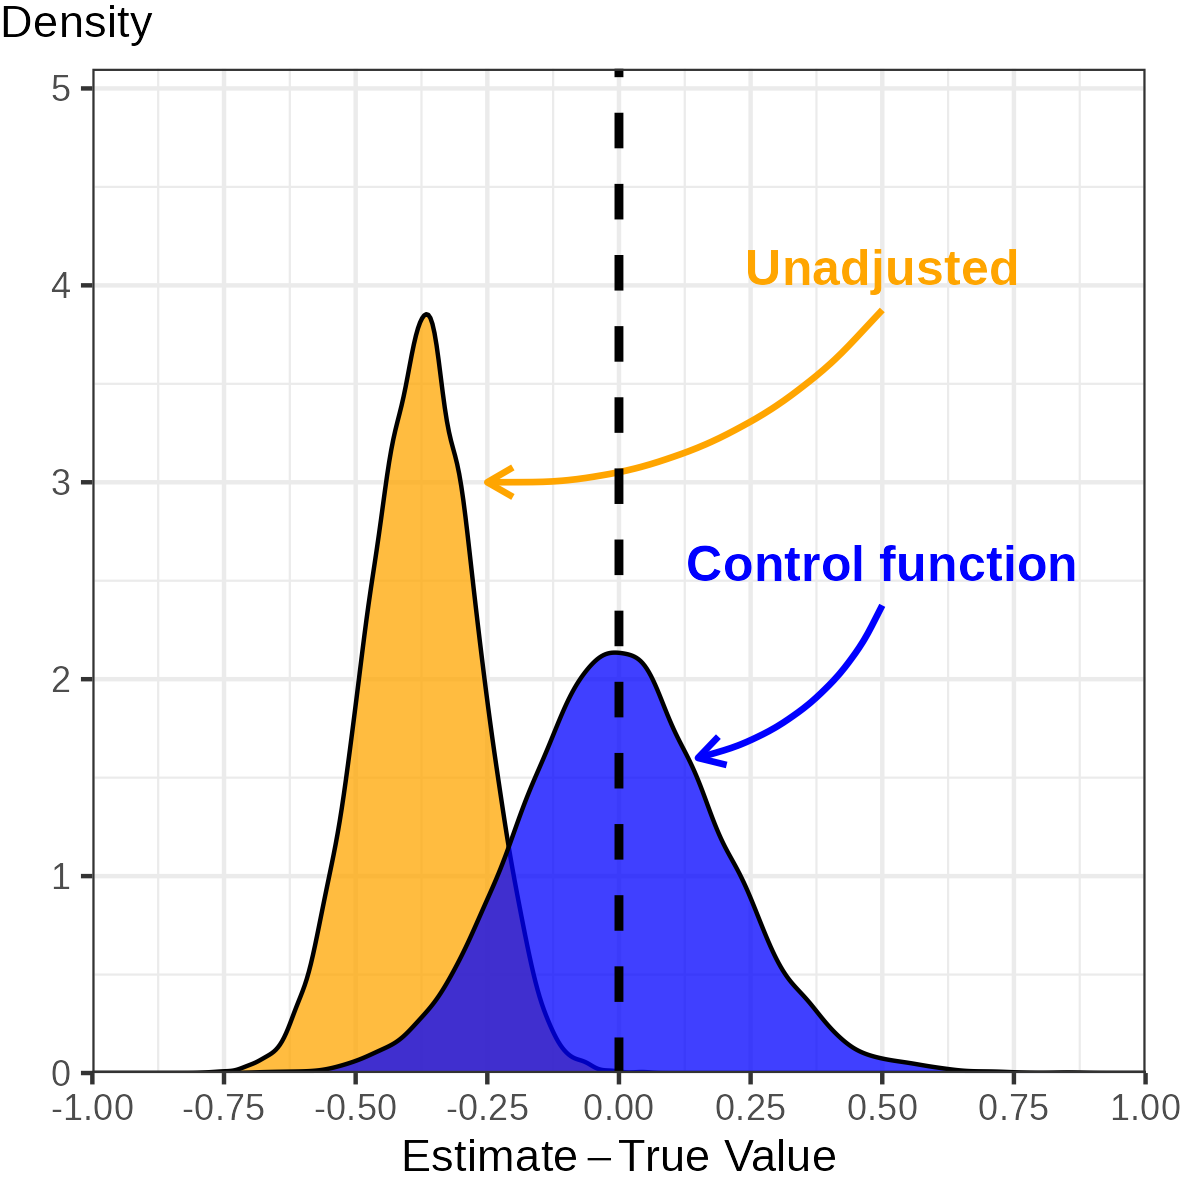
\includegraphics[width=\textwidth]{
            ../programs/simulations/sim-output/heckit-direct-dist.png}
    \end{subfigure}
    \begin{subfigure}[c]{0.475\textwidth}
        \centering
        \caption{$\hat{\text{AIE}} - \text{AIE}$.}
        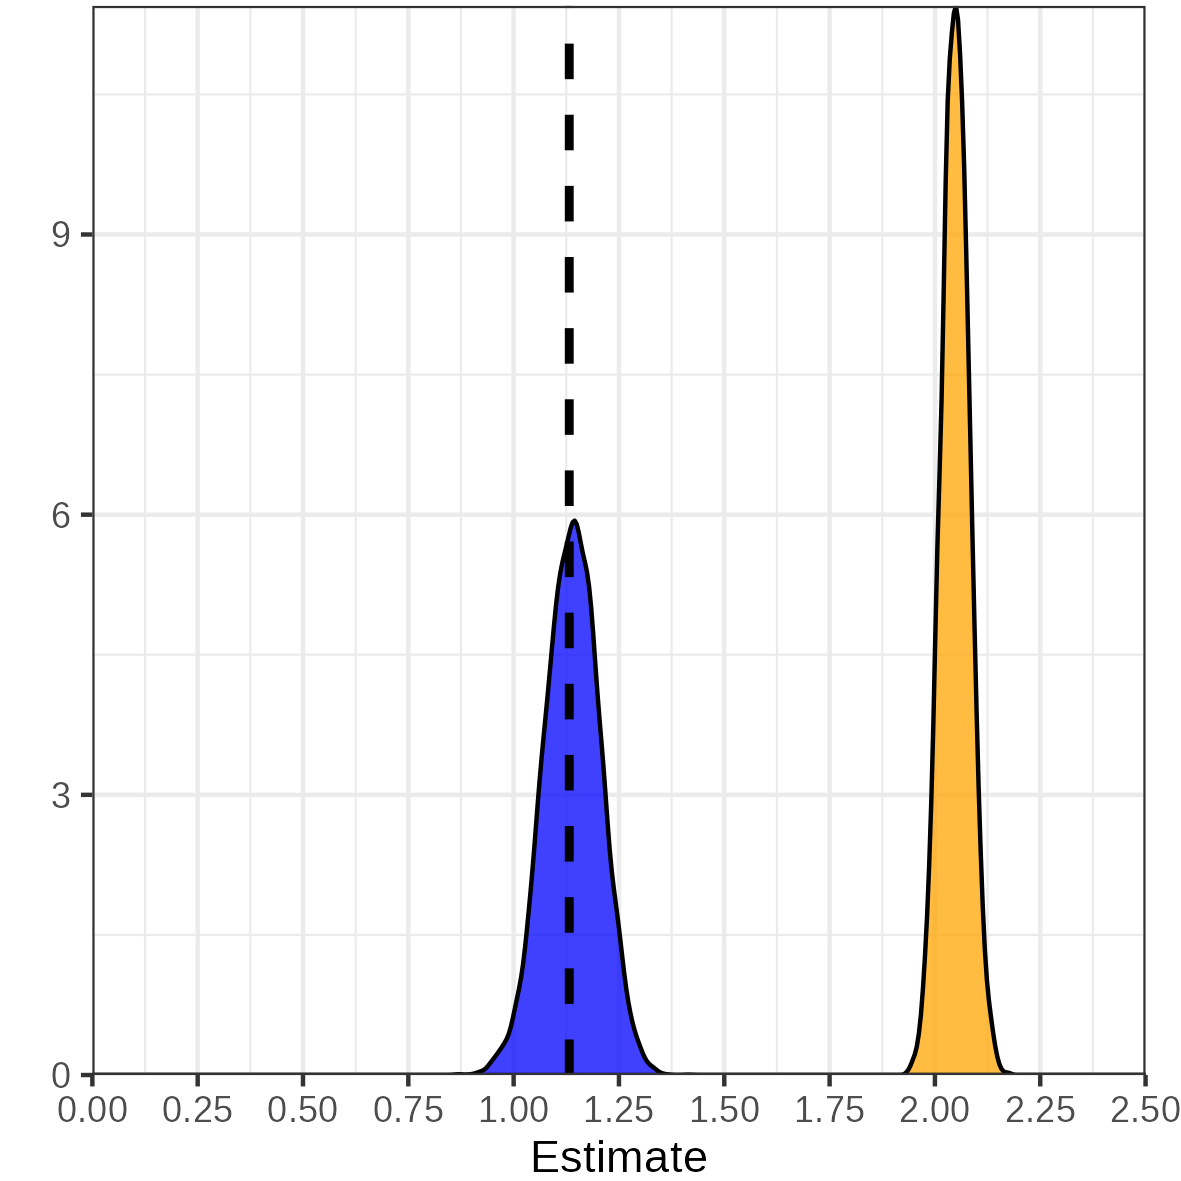
\includegraphics[width=\textwidth]{
            ../programs/simulations/sim-output/heckit-indirect-dist.png}
    \end{subfigure}
    \label{fig:cm-heckit-dist}
    \justify
    \footnotesize    
    \textbf{Note:}
    These figures show the empirical density of point estimates minus the true average effect, for 10,000 different datasets generated from a Roy model with correlated normally distributed error terms (further described in \autoref{sec:simulations}).
    The black dashed line is the true value;
    orange is the distribution of conventional CM estimates from two-stage OLS \citep{imai2010identification},
    and blue estimates with a two-stage Heckman selection adjustment.
\end{figure}

\autoref{fig:cm-heckit-dist} shows how a CF adjustment corrects unadjusted CM effect estimates.
In a simulation with selection-into-mediator based on unobserved error terms, the CF adjustment pushes conventional CM estimates back to the true value. 

% \subsubsection{Connection to Marginal Treatment Effects}
% It is worth noting that this approach is essentially an MTE approach (Marginal Treatment Effect, developed by Heckman and Vytlacil, 1999, 2005) applied to a causal mediation setting. Just as the semi-parametric local IV approach uses variation in instruments to identify marginal treatment effects across different resistance-to-treatment margins, our semi-parametric CF approach identifies mediation effects across the distribution of unobserved mediator gains. This connection to the MTE literature provides a conceptual bridge between the instrumental variables literature and causal mediation analysis.

% Model-based Framework, mediation under Roy-style selection
\section{Control Function (CF) Estimation of CM Effects}
\label{sec:controlfun}
A conventional approach to estimating CM effects involves a two-stage approach to estimating the ADE and the AIE: the first-stage $Z \to D$ and the second-stage $Z, D \to Y$.
A CF approach is a simple and intuitive addition to this approach: including the CF terms $\lambda_0, \lambda_1$ in the second-stage regression to address selection-into-mediator.

This section presents two practical estimation strategies.
First, I demonstrate how to estimate CM effects with an assumed distribution of error terms, focusing on the Heckman selection model as the leading case.
Second, I consider a more flexible semi-parametric approach that avoids distributional assumptions --- at the cost of semi-parametrically estimating the corresponding CFs.
While both methods effectively address the selection bias issues detailed in previous sections, they differ in their implementation complexity, efficiency, and underlying assumptions.

\subsection{Parametric CF}
A parametric CF solves the identification problem by assuming a distribution for the unobserved error terms in the first-stage selection model, and modelling selection based on this distribution.
The Heckman selection model is the most pertinent example, assuming the normal distribution for unobserved errors \cite{heckman1979sample}.
A parametric CF using other distributions works in exactly the same manner, replacing the relevant density functions for an alternative distribution as needed.
As such, this section focuses exclusively on the Heckman selection model.

The Heckman selection model assumes unobserved errors $V_i$ follow a normal distribution, so estimates the first-stage using a probit model.
\[ \Probgiven{D_i = 1}{Z_i, \vec X_i}
    = \Phi \big( \phi + \bar\pi Z_i + \vec\zeta' \vec X_i \big), \]
where $\Phi(.)$ is the cumulative density function for the normal distribution, and $\phi, \bar\pi, \vec\zeta$ are parameters estimated with maximum likelihood.

From this probit first-stage, we construct an estimate of the inverse Mills ratio terms to serve as the CFs.
These terms capture the correlation between unobserved factors influencing both mediator selection and outcomes, when the errors are normally distributed.
\[ \hat \lambda_0 = 1 - \Phi^{-1} \left( \hat\phi + \hat{\bar\pi} Z_i + \hat{\vec\zeta}' \vec X_i \right), \;\;\;\;
\hat \lambda_1 = \Phi^{-1} \left( \hat\phi + \hat{\bar\pi} Z_i + \hat{\vec\zeta}' \vec X_i \right). \]
Lastly, the second-stage is estimated with OLS, including the estimated CFs,
\[ Y_i = \alpha + \beta D_i + \gamma Z_i + \delta Z_i D_i + \vec\varphi' \vec X_i^- 
    + \rho_0(1-D_i) \hat \lambda_0 + \rho_1 D_i \hat \lambda_1 + \varepsilon_i. \]
The resulting ADE and AIE estimates are composed from sample estimates of the terms in Theorem \ref{thm:cf-identification},
\[ \hat{\text{ADE}}
    = \hat{\gamma} + \hat{\delta}\,\bar D_i, \;\;\;\;
    \hat{\text{AIE}}
    = \hat{\bar\pi}\; \Big(
        \hat{\beta} + \hat{\delta}\,\bar Z_i 
        + \big(\hat \rho_1 - \hat \rho_0 \big)
        \hat \Gamma \big( \hat\pi(0;\vec X_i), \hat\pi(1;\vec X_i)\big) \Big) \]
where $\bar D_i = \frac1N \sum_{i=1}^N D_i$, $\bar Z_i = \frac1N \sum_{i=1}^N Z_i$, and $\hat\pi \big(z';\vec X_i \big) = \Phi \big( \hat\phi + \hat{\bar\pi} z' + \hat{\vec\zeta}' \vec X_i \big)$ are the predictions for the probit first-stage, and $\hat\Gamma(.,.)$ is the estimate of the complier adjustment term using the estimated CF, $\hat\lambda_1$.

The standard errors for estimates can be computed using the delta method \citep{heckman1979sample}.
Specifically, we account for both the sampling variability in the coefficient estimates and the fact that the CFs themselves are estimated in the first-stage.
This approach yields $\sqrt{n}$-consistent estimates when the underlying error terms follow a bivariate normal distribution --- i.e., when $\lambda_0, \lambda_1$ and $\hat\pi$ are correctly modelled by the probit first-stage.
Errors can also be estimated by the bootstrap, including estimation of both the first and second-stage within each bootstrap iteration.

In practice, a parametric CF approach is simple to implement using standard statistical packages.
The key advantage is computational simplicity and efficiency, particularly in moderate-sized samples.
However, this comes at the cost of strong distributional assumptions.
For example, if the error terms deviate substantially from joint normality, the estimates may be biased.

\subsection{Semiparametric CF}
For settings where researchers are not comfortable specifying a specific distribution for the error terms, a semiparametric CF will nonetheless consistently estimate CM effects.
This method maintains the same identification strategy but avoids assuming a specific parametric error distribution.

The semiparametric approach begins with flexible estimation of the first-stage, non-parametrically estimating the mediator propensity score,
%\begin{equation}
%    \label{eqn:nonparametric-firststage}
\[ \pi\left(Z_i; \vec X_i \right) = \Egiven{D_i}{Z_i, \vec X_i}, \]
%\end{equation}
where $\vec X_i$ must include the instrument(s) $\vec X_i^{\text{IV}}$.
This can be estimated using flexible methods such as series approximation or kernel-based approaches, as long as the first-stage is estimated $\sqrt{n}$-consistently.\footnote{
    If an estimate of the first-stage that is not $\sqrt{n}$-consistent is used (e.g., a modern machine learning estimator), then the resulting second-stage estimate will not be $\sqrt{n}$-consistent.
    This could be ameliorated by augmenting the approach with cross-fitting, and the appropriate Neyman orthogonal moments; \cite{bia2024double} use this approach for one-sided selection problems, but (as fas as I am aware) there is no general double machine learning approach for CF methods for two-sided selection problems.  
}

Next the CFs, themselves, are estimated with semi-parametric methods.
Considering the $D_i = 0$ subsample first.
\[ \Egiven{Y_i}{Z_i, D_i = 0, \vec X_i} =
    \alpha + \gamma Z_i + \varphi\big( \vec X_i^- \big)
    +  \left( 1 - D_i \right) \rho_0 \lambda_0 \big( \pi(Z_i ; \vec X_i) \big), \]
which gives a regression equation to estimate semi-parametrically, with the first-estimate estimate $\hat\pi\left(Z_i; \vec X_i \right)$ plugged in.
The linear parameters ($\alpha, \gamma$ and a linear approximation of control parameter $\varphi$) can be estimated with OLS, with appropriate interactions to flexibly control for $\vec X_i$, and $\lambda_0$ with a flexible semiparametric specification.
An attractive option is a flexible series estimation, such as a spline specification, as this flexibly estimates the function without assuming a functional form but maintains $\sqrt n$-consistency.
Note that $\lambda_0$ can no longer be separated from $\rho_0$ in this semi-parametric approach; the complier adjustment term requires $\rho_0, \rho_1$ only be identified up to a constant.
Next, the $\rho_0 \lambda_0$ function is extrapolated to the $D_i = 1$ side, identifying the remaining terms $\beta, \delta$, and thus the ADE and AIE.\footnote{
    \aref{appendix:semiparametric} explains these points in further detail.
}

Return to the $D_i = 1$ subsample,
\[ \Egiven{Y_i}{Z_i, D_i = 1, \vec X_i} =
    (\alpha + \beta) + (\gamma + \delta) Z_i + \varphi\big( \vec X_i^- \big)
    +  D_i \rho_1 \lambda_1 \big( \pi(Z_i ; \vec X_i) \big). \]
The same process extrapolates the series estimate of $\rho_1 \lambda_1$ to the $D_i = 0$ subsample, for another set of estimates for the ADE and AIE.
An efficient estimate can compose these two estimates of the CM effects, with weights proportional to the efficiency of each side.

This approach achieves valid estimation of the CM effects, without specifying the distribution behind unobserved error terms, and achieves desirable properties as long as the first-stage correctly estimates the mediator propensity score, and the structural assumptions hold true.
The standard errors for estimates can again be computed using the delta method, or estimated by the bootstrap --- again, across both first and second-stages within each bootstrap iteration.
Note that relying on propensity score estimation requires assumptions that can be found wanting in real-world settings; a common support condition for the mediator is required, and the semiparametric first-stage may become cumbersome if there are many control variables.

%\subsection{Validation of the CF assumptions via 2SLS}
%If the structural assumptions hold, then a 2SLS for $D \to Y$, using $\vec X^{\text{IV}}$ should give the same as a CF estimate.
%If not, then a violation of the structural assumptions somewhere.
%Could be put into an informal hypothesis test, where the null $\beta^\text{IV} = \beta^\text{CF}$ could be rejected.

%\subsection{Percent of ATE Mediated Through $D$}
%It is common to focus on AIE / ATE, which is necessarily a noisy estimate.
%Indeed, the Kwon Roth gives a test to validate (though not confirm) that everything goes through AIE.
%If reject, then move forward with this.
%
%An inverse variance weighted version of AIE / ATE, which efficiently uses (1) AIE estimate (2) a function of the ADE estimate.
%This addresses some of the inefficiency in estimating this term.
%
%If you have large uncertainty in your treatment effect, then expect large uncertainty in the mechanisms behind it.
%There is no avoiding the fact that a noisy ATE estimate (especially if close to zero) will mean noisy estimates of AIE / ATE.  

\subsection{Simulation Evidence}
\label{sec:simulations}
The following simulation gives an example to show how these methods work in practice.
Suppose data observed to the researcher $Z_i, D_i, Y_i, \vec X_i$ are drawn from the following data generating processes, for $i = 1, \hdots, N$, with 
$N = 1,000$ for this simulation.
\[ Z_i \sim \text{Binom}\left(0.5 \right),
    \;\; \vec X_i^- \sim N(4, 1),
    \;\; \vec X_i^{\text{IV}} \sim \text{Binom}\left( 0.5 \right),
    \;\; \left( U_{0,i}, U_{1,i}, U_{C,i} \right) \sim
    N\left( \vec 0, \mat \Sigma \right) \]

Each $i$ chooses to take mediator $D_i$ by a Roy model, with following mean definitions for each $z', d' = 0, 1$.
\begin{align*}
    D_i(z') = \indicator{Y_i(z', 1) - Y_i(z', 0) \geq C_i},  \\
    \mu_{d'}\left(z' ; \vec X_i \right) = \vec X_i^- + \left( z' + d' + z' d' \right),
    \;\; \mu_{C}\left(z' ; \vec X_i \right) = 3z' + \vec X_i^- - \vec X_i^{\text{IV}}.
\end{align*}
Following \autoref{sec:applied}, these data have the following first and second-stage equations:
\begin{align*}
    D_i &= \indicator{-3Z_i - \vec X_i^{\text{IV}} + \vec X_i^-
        \geq U_{C,i} - \big( U_{1,i} - U_{0,i} \big)},  \\
    Y_i &= Z_i + D_i + Z_i D_i + \vec X_i^-
        + \left( 1 - D_i \right) U_{0,i} + D_i U_{1,i}.
\end{align*}
$Z_i$ has an effect on outcome $Y_i$, and it operates partially through mediator $D_i$.
Outcome mean $\mu_{D_i}(Z_i;.)$ contains an interaction term, $Z_i D_i$, so while both $Z_i$ and $D_i$ have constant partial effects, the ATE depends on how many $i$ choose to take the mediator.
In this simulation $\Prob{D_i = 1} = 0.437$, and $65.29\%$ of the sample are mediator compliers (where $D_i(1)=1$ and $D_i(0) = 0$).
This gives an ATE ($Z\to Y$) value of 2.58, ADE 1.44, and AIE 1.13, respectively.\footnote{
    Note that ATE $=$ ADE $+$ AIE in this setting.
    $\Prob{Z_i=1} = 0.5$ ensures this equality, but it is not guaranteed in general.
}

After $Z_i$ is assigned, $i$ chooses to take mediator $D_i$ by considering the costs and benefits --- which vary based on $Z_i$, demographic controls $\vec X_i$, and the (non-degenerate) unobserved error terms $U_{i,0}, U_{1,i}$.
As a result, sequential ignorability does not hold; the mediator is not conditionally ignorable.
Thus, a standard OLS (selection-on-observables) approach to CM does not give an estimate for how much of the $Z \to Y$ ATE goes through mediator $D$.
Instead, the OLS approach gives biased inference.
The bias in OLS estimates comes from the unobserved error terms being related.

\begin{figure}[h!]
    \caption{Simulated Distribution of CM Effect Estimates, Semi-parametric versus OLS, Relative to True Value.}
    \begin{subfigure}[c]{0.475\textwidth}
        \centering
        \caption{$\hat{\text{ADE}} - \text{ADE}$.}
        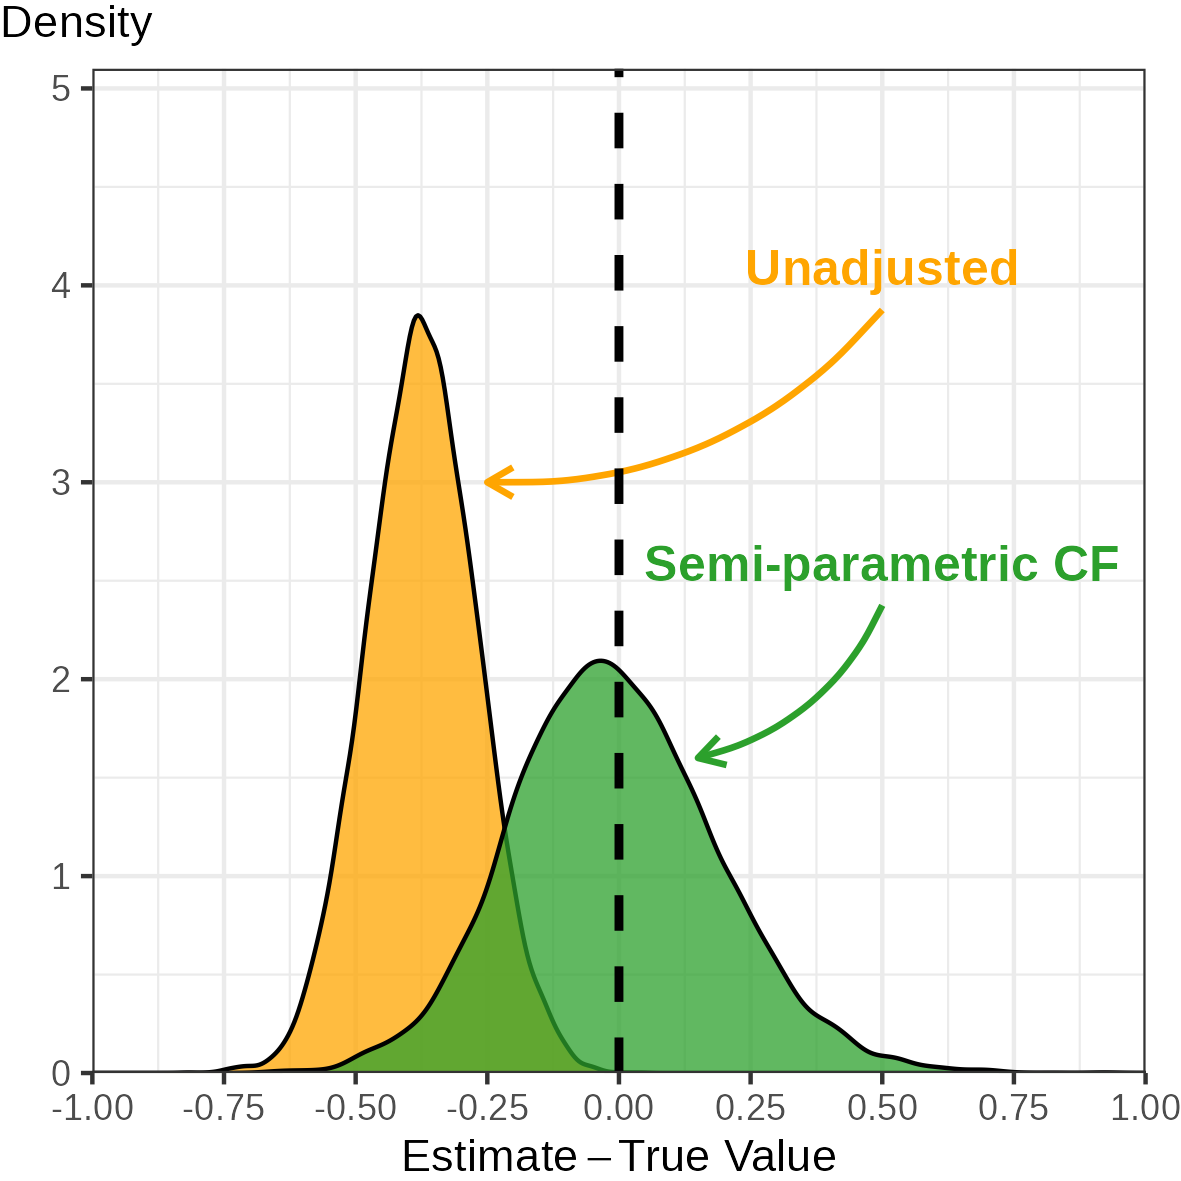
\includegraphics[width=\textwidth]{
            ../programs/simulations/sim-output/semiparametric-direct-dist.png}
    \end{subfigure}
    \begin{subfigure}[c]{0.475\textwidth}
        \centering
        \caption{$\hat{\text{AIE}} - \text{AIE}$.}
        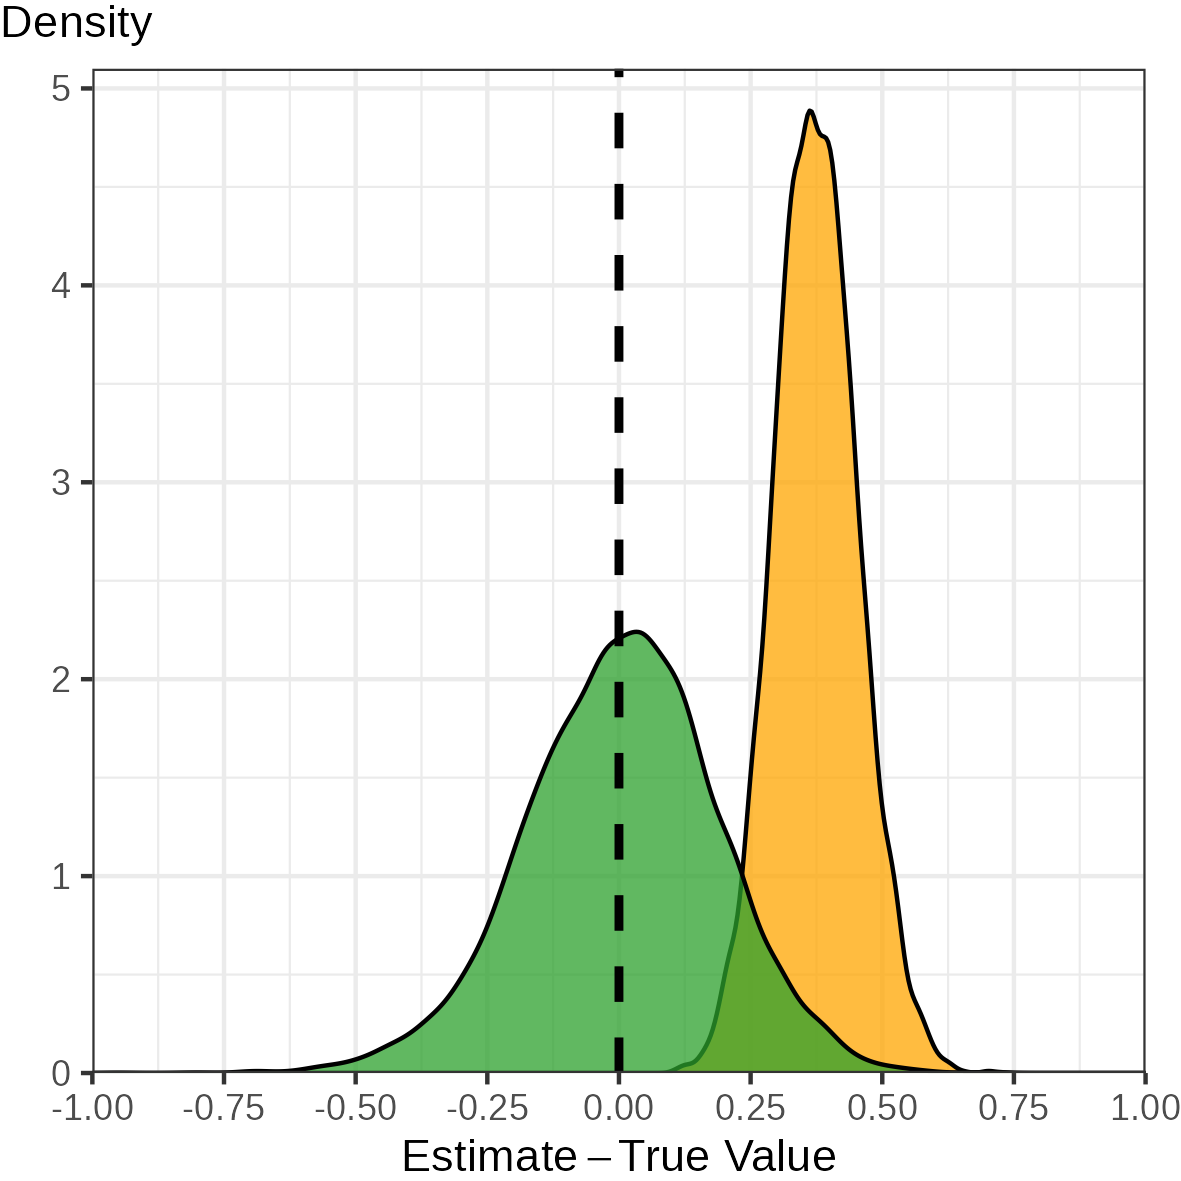
\includegraphics[width=\textwidth]{
            ../programs/simulations/sim-output/semiparametric-indirect-dist.png}
    \end{subfigure}
    \label{fig:cm-semiparametric-dist}
    \justify
    \footnotesize    
    \textbf{Note:}
    These figures show the empirical density of point estimates minus the true average effect, for 10,000 different datasets generated from a Roy model with correlated normally distributed error terms (further described in \autoref{sec:controlfun}).
    The black dashed line is the true value;
    orange is the distribution of conventional CM estimates from two-stage OLS \citep{imai2010identification},
    and green estimates with a two-stage semi-parametric CF.
\end{figure}

The CF estimator here uses the inverse Mills ratio as the CFs (i.e., a Heckman selection model); the constrained semi-parametric approach explcitily models $\lambda_1$ , and thus $\lambda_0$, with data to avoid distributional assumptions.
\autoref{fig:cm-semiparametric-dist} shows the distribution of simulated point estimates in this simulation, showing OLS against the CF approach.
The OLS approach implicitly assumes that the mediator is ignorable (when it is not), so its point estimates under and over-estimate the true ADE and AIE, respectively.
The distance between the OLS estimates and the true values are the underlying bias terms derived in \autoref{thm:selection-bias}.
In this data generating process, the OLS confidence interval do not overlap the true values for any standard level of significance.
The CF approach exhibits bias, though the 95\% confidence intervals cover the truth.

\begin{figure}[h!]
    \caption{Point Estimates of CM Effects, OLS versus CF, varying $\rho$ values with $\sigma_0 = 1, \sigma_1 = 2$ fixed.}
    \begin{subfigure}[c]{0.475\textwidth}
        \centering
        \caption{ADE.}
        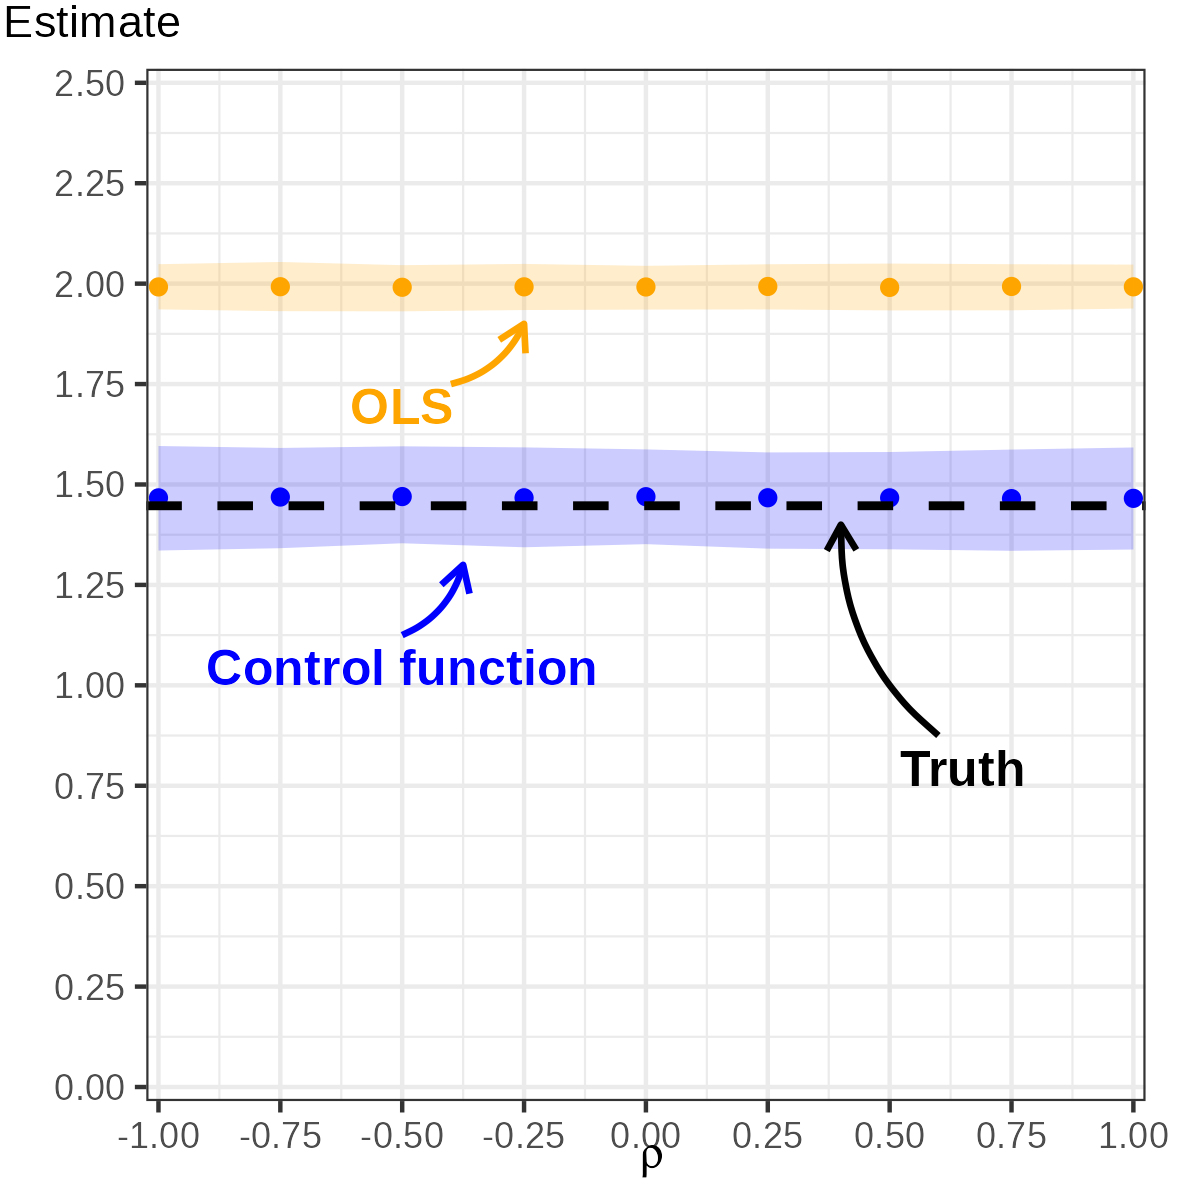
\includegraphics[width=\textwidth]{
            ../programs/simulations/sim-output/rho-directeffect-bias.png}
    \end{subfigure}
    \begin{subfigure}[c]{0.475\textwidth}
        \centering
        \caption{AIE.}
        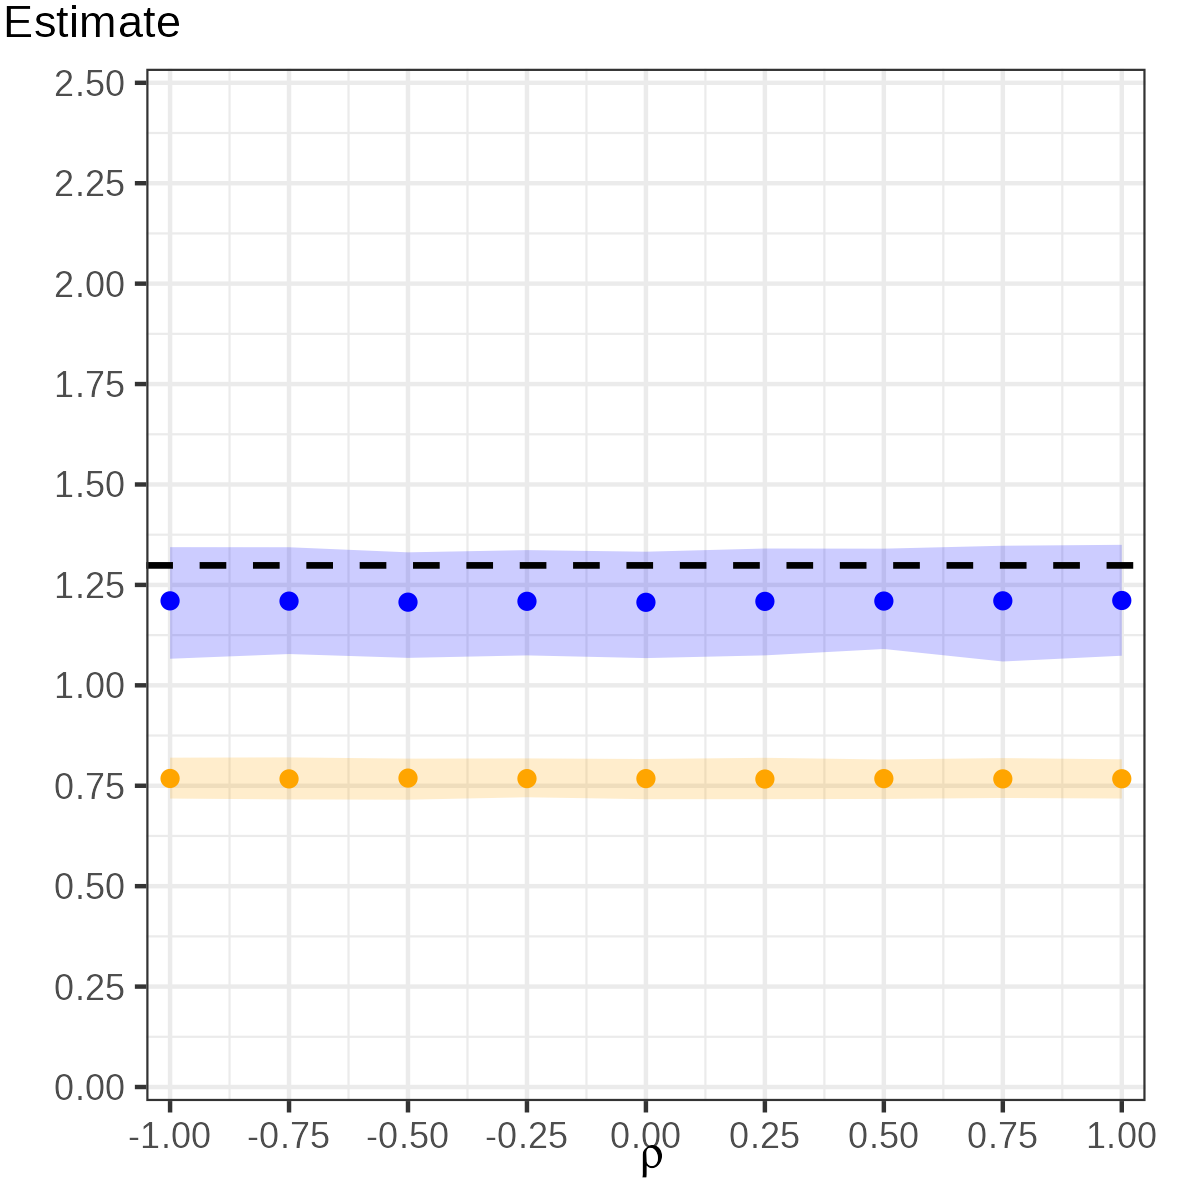
\includegraphics[width=\textwidth]{
            ../programs/simulations/sim-output/rho-indirecteffect-bias.png}
    \end{subfigure}
    \label{fig:rho-bias}
    \justify
    \footnotesize    
    \textbf{Note:}
    These figures show the OLS and CF point estimates of the ADE and AIE, for $N = 10,000$ sample size.
    The black dashed line is the true value, points are points estimates from data simulated with a given $\rho$ value and $\sigma_0 = 1, \sigma_1 = 2$, and shaded regions are the 95\% confidence intervals from 1,000 bootstraps each.
    Orange represents OLS estimates, blue the CF approach.
    The true AIE values vary with $\rho$, because $D_i(Z_i)$ compliers have higher average values of $U_{1,i} - U_{0,i}$ with greater $\rho$ values.
\end{figure}

The error terms determine the bias in OLS estimates of the ADE and AIE, so the bias varies for different values of the error-term parameters $\rho \in [-1, 1]$ and $\sigma_0, \sigma_1 \geq 0$.
\autoref{fig:rho-bias} shows CF estimates against estimates calculated by standard OLS, showing 95\% confidence intervals calculated from 1,000 bootstraps.
The point estimates of the CF do not exactly equal the true values, as they are estimates from one simulation (not averages across many simulations, as in \autoref{fig:cm-semiparametric-dist}).
The CF approach improves on OLS estimates by correcting for bias, with confidence regions overlapping the true values.\footnote{
    In the appendix, \autoref{fig:sigma-bias} shows the same simulation while varying $\sigma_1$, with fixed $\sigma_0 = 1, \rho = 0.5$.
    The conclusion is the same as for varying the correlation coefficient, $\rho$, in \autoref{fig:rho-bias}.
}
This correction did not come for free: the standard errors are significantly greater in a CF approach than OLS.
Standard errors on the AIE are larger than those for the ADE, because the AIE estimates are first-stage times second-stage estimates, so standard errors account for uncertainty in both estimates multiplied.
%(i.e., the same reasons instrumental variables estimates are less efficient than ideal OLS estimates). 
In this manner, this simulation shows the pros and cons of using the CF approach to estimating CM effects in practice.

% Conclusion Section
%%%%%%%%%%%%%%%%%%%%%%%%%%%%%%%%%%%%%%%%%
%% Conclusion section
\section{Summary and Concluding Remarks}
\label{sec:conclusion}

This paper has studied a selection-on-observables approach to CM in a natural experiment setting.
I have shown the pitfalls of using the most popular methods for estimating direct and indirect effects without a clear case for the mediator being ignorable.
Using the Roy model as a benchmark, a mediator is unlikely to be ignorable in natural experiment settings, and the bias terms likely crowd out inference regarding CM effects.

This paper has contributed to the growing CM literature in economics, integrating labour economic theory for select-into-treatment as a way of judging CM methods.
It has drawn on the classic literature, and pointed to already-in-use control function methods as a compelling way of estimating direct and indirect effects in a natural experiment setting.
Further research could build on this approach by suggesting efficiency improvements, adjustments for common statistical irregularities (say, cluster dependence), or integrating the control function as an additional robustness in the growing double robustness literature \citep{huber2019review,bia2024double}.

This paper has not lit the way for applied researchers to use CM methods unabashedly, with or without a control function adjustment.
The structural assumptions are strong and large sample sizes are needed; if the assumptions are broken, then the control function method does not improve on a na\"ive selection-on-observables approach to CM estimates.
And yet, there are likely settings in which the structural assumptions are credible.
Mediator monotonicity aligns well with economic theory in many cases, and it is plausible for researchers to study big data settings with exogenous variation in mediator take-up costs.
In these cases, this paper opens the door to identifying mechanisms behind treatment effects in natural experiment settings.
% The approach could be used in AB tests, where a firm randomises a treatment and costs of a suspected mediator (if they do not want to also randomise a mediator fully).


% Bibliography
\singlespacing
\bibliographystyle{agsm}
\bibliography{sections/07-bibliography.bib}
% Appendix
\newpage
%%%%%%%%%%%%%%%%%%%%%%%%%%%%%%%%%%%%%%%%%
%% Appendix section
% Set-up the section.
%\newpage
\onehalfspacing
\appendix
\setcounter{table}{0}
\renewcommand{\thetable}{A\arabic{table}}
\setcounter{figure}{0}
\renewcommand{\thefigure}{A\arabic{figure}}

% Start appendix
\section{Supplementary Appendix}
\label{appendix}
This section is for supplementary information, and validation of presented propositions and theorems.
It is not meant for publication.

Any comments or suggestions may be sent to me at \href{mailto:seh325@cornell.edu}{\nolinkurl{seh325@cornell.edu}},
or raised as an issue on the Github project,
\url{https://github.com/shoganhennessy/mediation-natural-experiment}.

%\subsection{Previous Literature}
%\label{appendix:mediation-review}
%
%Create a table in this section that surveys previous research which employs mediation methods while having a clear causal design for $Z_i$, but not $D_i$.
%
%\begin{tabular}{l l l l l}
%    Paper & Field & Research Design for $Z_i$ & Research Design for $D_i$ & Selection bias? \\ \hline
%    Paper name 1.    
%\end{tabular}


\subsection{Identification in Causal Mediation}
\label{appendix:identification}
\citet[Theorem~1]{imai2010identification} states that the ADE and AIE are identified under sequential ignorability, at each level of $Z_i = 0,1$.
For $z' = 0,1$: \\
\makebox[\textwidth]{\parbox{1.25\textwidth}{
\begin{align*}
    \E{ Y_i(1, D_i(z')) - Y_i(0, D_i(z'))}
    &= \int \int 
    \Big( \Egiven{ Y_i }{Z_i = 1, D_i, \vec X_i}
        - \Egiven{ Y_i }{Z_i = 0, D_i, \vec X_i} \Big)
            dF_{D_i \, | \, Z_i = z', \vec X_i} dF_{\vec X_i}, \\
    \E{ Y_i(z', D_i(1)) - Y_i(z', D_i(0))}
    &= \int \int \Egiven{ Y_i }{Z_i = z', D_i, \vec X_i}
    \Big( dF_{D_i \, | \, Z_i = 1, \vec X_i}
        - dF_{D_i \, | \, Z_i = 0, \vec X_i} \Big) dF_{\vec X_i}.
\end{align*}
}}
I focus on the averages, which are identified by consequence of the above.
\begin{align*}
    \E{ Y_i(1, D_i(Z_i)) - Y_i(0, D_i(Z_i))}
    &= \E[Z_i]{\Egiven{ Y_i(1, D_i(z')) - Y_i(0, D_i(z'))}{Z_i = z'}} \\
    \E{ Y_i(Z_i, D_i(1)) - Y_i(Z_i, D_i(0))}
    & = \E[Z_i]{\Egiven{ Y_i(z', D_i(1)) - Y_i(z', D_i(0))}{Z_i = z'}}
\end{align*}
My estimand for the ADE is a simple rearrangement of the above.
The estimand for the AIE relies on a different sequence, relying on (1) sequential ignorability, (2) conditional monotonicity.
These give (1) identification equivalence of AIE local to cpmpliers conditional on $\vec X_i$ and AIE conditional on $\vec X_i$, LAIE $=$ AIE, (2) identification of the complier score.
%, $\Probgiven{D_i(0) = 0, D_i(1) = 1}{\vec X_i}$ $= \Egiven{Y_i}{Z_i, D_i = 1, \vec X_i}
%- \Egiven{Y_i}{Z_i, D_i = 0, \vec X_i}$.
\begin{align*}
    & \Egiven{ Y_i(Z_i, D_i(1)) - Y_i(Z_i, D_i(0))}{\vec X_i} \\
    & = \Probgiven{D_i(0) = 0, D_i(1) = 1}{\vec X_i}
        \Egiven{ Y_i(Z_i, 1) - Y_i(Z_i, 0)}{D_i(0) = 0, D_i(1) = 1, \vec X_i} \\
    & = \Probgiven{D_i(0) = 0, D_i(1) = 1}{\vec X_i}
        \Egiven{ Y_i(Z_i, 1) - Y_i(Z_i, 0)}{\vec X_i} \\
    & = \Probgiven{D_i(0) = 0, D_i(1) = 1}{\vec X_i}
        \; \Big( \Egiven{Y_i}{Z_i, D_i = 1, \vec X_i}
            - \Egiven{Y_i}{Z_i, D_i = 0, \vec X_i} \Big) \\
    & = \Big( \Egiven{D_i}{Z_i = 1, \vec X_i} - \Egiven{D_i}{Z_i = 0, \vec X_i}
        \Big) \;
        \Big( \Egiven{Y_i}{Z_i, D_i = 1, \vec X_i}
            - \Egiven{Y_i}{Z_i, D_i = 0, \vec X_i} \Big)
\end{align*}
Monotonicity is not technically required for the above.
Breaking monotonicity would not change the identification in any of the above; it would be the same except replacing the complier score with a complier/defier score, $\Probgiven{D_i(0) \neq D_i(1)}{\vec X_i} = \Egiven{D_i}{Z_i = 1, \vec X_i} - \Egiven{D_i}{Z_i = 0, \vec X_i}$.

%\subsection{Continuous Average Causal Responses}
%\label{appendix:continuous}
%Section here relating the approach to the average causal response function (see e.g., Angrist Imbens JASA 1996, Andrew Bacon for DiD 2023).

% \subsection{Previous Literature}
% \label{appendix:mediation-review}
% 
% Create a table in this section that surveys previous research which employs mediation methods while having a clear causal design for $Z_i$, but not $D_i$.
%
%\begin{tabular}{l l l l l}
%    Paper & Field & Research Design for $Z_i$ & Research Design for $D_i$ & Selection bias? \\ \hline
%    Paper name 1.    
%\end{tabular}

\subsection{Bias in Causal Mediation (CM) Estimands}
\label{appendix:mediation-bias}
Suppose that $Z_i$ is ignorable conditional on $\vec X_i$, but $D_i$ is not.

\subsubsection{Bias in the Average Direct Effect (ADE)}
To show that the conventional approach to mediation gives an estimate for the ADE with selection and group difference-bias, start with the components of the conventional estimands.
This proof starts with the relevant expectations, conditional on a specific value of $\vec X_i$ and $d' \in \{0, 1 \}$.
\begin{align*}
    \Egiven{Y_i}{Z_i = 1, D_i = d', \vec X_i}
    =& \Egiven{Y_i(1, D_i(Z_i))}{D_i(1) = d', \vec X_i}, \\
    \Egiven{Y_i}{Z_i = 0, D_i = d', \vec X_i}
    =& \Egiven{Y_i(0, D_i(Z_i))}{D_i(0) = d', \vec X_i}
\end{align*}
And so,
\begin{align*}
    &  \Egiven{Y_i}{Z_i = 1, D_i = d', \vec X_i}
    - \Egiven{Y_i}{Z_i = 0, D_i = d', \vec X_i} \\
    &= \Egiven{Y_i(1, D_i(Z_i))}{D_i(1) = d', \vec X_i}
    - \Egiven{Y_i(0, D_i(Z_i))}{D_i(0) = d', \vec X_i} \\
    &= \Egiven{Y_i(1, D_i(Z_i)) - Y_i(0, D_i(Z_i))}{D_i(1) = d', \vec X_i} \\
    &\;\;\;\;+ \Egiven{Y_i(0, D_i(Z_i))}{D_i(1) = d', \vec X_i}
        - \Egiven{Y_i(0, D_i(Z_i))}{D_i(0) = d', \vec X_i}.
\end{align*}
The final term is a sum of the ADE, conditional on $D_i(1) = d'$, and a selection bias term --- difference in baseline outcomes between the (partially overlapping) groups for whom $D_i(1) = d'$ and $D_i(0) = d'$.

To reach the final term, note the following.
\begin{align*}
    &\Egiven{Y_i(1, D_i(Z_i)) - Y_i(0, D_i(Z_i))}{\vec X_i} \\    
    &= \Egiven{Y_i(1, D_i(Z_i)) - Y_i(0, D_i(Z_i))}{D_i(1) = d', \vec X_i} \\
    &\;\;\;\;+ \Big(1 - \Probgiven{D_i(1) = d'}{\vec X_i}\Big)
    \left( \begin{aligned}
        &\Egiven{Y_i(1, D_i(Z_i)) - Y_i(0, D_i(Z_i))}{D_i(1) = d', \vec X_i} \\ 
        & - \Egiven{Y_i(1, D_i(Z_i)) - Y_i(0, D_i(Z_i))}{D_i(1) = 1 - d', \vec X_i}
    \end{aligned} \right) 
\end{align*}
The second term is the difference between the ADE and LADE local to relevant complier groups.

Collect everything together, as follows.
\begin{align*}
    &  \Egiven{Y_i}{Z_i = 1, D_i = d', \vec X_i}
    - \Egiven{Y_i}{Z_i = 0, D_i = d', \vec X_i} \\
    =& \underbrace{
        \Egiven{Y_i(1, D_i(Z_i)) - Y_i(0, D_i(Z_i))}{\vec X_i}}_{
            \text{ADE, conditional on }\vec X_i} \\
    &+ \underbrace{
        \Egiven{Y_i(0, D_i(Z_i))}{D_i(1) = d', \vec X_i}
            - \Egiven{Y_i(0, D_i(Z_i))}{D_i(0) = d', \vec X_i}}_{
                \text{Selection bias}} \\
    &+ \underbrace{\Big(1 - \Probgiven{D_i(1) = d'}{\vec X_i}\Big)
    \left( \begin{aligned}
        &\Egiven{Y_i(1, D_i(Z_i)) - Y_i(0, D_i(Z_i))}{D_i(1) = 1 - d', \vec X_i} \\ 
        & - \Egiven{Y_i(1, D_i(Z_i)) - Y_i(0, D_i(Z_i))}{D_i(1) = d', \vec X_i}
    \end{aligned} \right)}_{
        \text{group difference-bias}}
\end{align*}
The proof is achieved by applying the expectation across $D_i = d'$, and $\vec X_i$.

\subsubsection{Bias in the Average Indirect Effect (AIE)}
To show that the conventional approach to mediation gives an estimate for the AIE with selection and group difference-bias, start with the definition of the ADE --- the direct effect among compliers times the size of the complier group.

This proof starts with the relevant expectations, conditional on a specific value of $\vec X_i$.
\begin{align*}
    &\Egiven{ Y_i(Z_i, D_i(1)) - Y_i(Z_i, D_i(0))}{\vec X_i} \\
    =& \Probgiven{D_i(0) = 0, D_i(1) = 1}{\vec X_i}
        \Egiven{ Y_i(Z_i, 1) - Y_i(Z_i, 0)}{D_i(0) = 0, D_i(1) = 1, \vec X_i}
\end{align*}
When $D_i$ is not ignorable, the bias comes from estimating the second term,
\\ $\Egiven{ Y_i(Z_i, 1) - Y_i(Z_i, 0)}{D_i(0) = 0, D_i(1) = 1, \vec X_i}$, the direct effect among mediator compliers.

Let $z' \in \{ 0, 1 \}$.
Again, note the mean outcomes in terms of average potential outcomes,
\begin{align*}
    \Egiven{Y_i}{Z_i = z', D_i = 1, \vec X_i}
    =& \Egiven{Y_i(z', 1)}{D_i = 1, \vec X_i}, \\
    \Egiven{Y_i}{Z_i = z', D_i = 0, \vec X_i}
    =& \Egiven{Y_i(z', 0)}{D_i = 0, \vec X_i}.
\end{align*}
So compose the selection bias term, as follows.
\begin{align*}
    & \Egiven{Y_i}{Z_i = z', D_i = 1, \vec X_i}
    - \Egiven{Y_i}{Z_i = z', D_i = 0, \vec X_i} \\
    =& \Egiven{Y_i(z', 1)}{D_i = 1, \vec X_i}
        - \Egiven{Y_i(z', 0)}{D_i = 0, \vec X_i} \\
    =& \Egiven{Y_i(z', 1) - Y_i(z', 0)}{D_i = 1, \vec X_i}
    + \Egiven{Y_i(z', 0)}{D_i = 1, \vec X_i} - \Egiven{Y_i(z', 0)}{D_i = 0, \vec X_i}
\end{align*}
The final term is a sum of the AIE, among the treated group $D_i = 1$, and a selection bias term --- difference in baseline potential outcomes between the groups for whom $D_i = 1$ and $D_i = 0$.

The AIE is the direct effect among compliers times the size of the complier group, so we need to compensate for the difference between the treated group $D_i = 1$ and complier group $D_i(0) = 0, D_i(1) = 1$.

Start with the difference between treated group's average and overall average.
\begin{align*}
    & \Egiven{Y_i(z', 1) - Y_i(z', 0)}{D_i = 1, \vec X_i} \\
    =& \Egiven{Y_i(z', 1) - Y_i(z', 0)}{\vec X_i} \\
    &+ \Big(1 - \Probgiven{D_i = 1}{\vec X_i} \Big)
    \left( \begin{aligned}
        &\Egiven{Y_i(z', 1) - Y_i(z', 0)}{D_i = 1, \vec X_i} \\ 
        &  - \Egiven{Y_i(z', 1) - Y_i(z', 0)}{D_i = 0, \vec X_i}
    \end{aligned} \right)
\end{align*}
Then the difference between the compliers' average and the overall average.
\begin{align*}
    & \Egiven{ Y_i(z', 1) - Y_i(z', 0)}{D_i(0) = 0, D_i(1) = 1, \vec X_i} \\
    =& \Egiven{Y_i(z', 1) - Y_i(z', 0)}{\vec X_i} \\
    & + \frac{1 - \Probgiven{D_i(0) = 0, D_i(1) = 1}{\vec X_i} }{
        \Probgiven{D_i(0) = 0, D_i(1) = 1}{\vec X_i}}
    \left( \begin{aligned}
        &\Egiven{Y_i(z', 1) - Y_i(z', 0)}{D_i(1) = 0 \text{ or } D_i(0)=1, \vec X_i} \\ 
        &  - \Egiven{Y_i(z', 1) - Y_i(z', 0)}{\vec X_i}
    \end{aligned} \right)
\end{align*}

Collect everything together, as follows.
\begin{align*}
    &  \Egiven{Y_i}{Z_i = z', D_i = 1, \vec X_i}
    - \Egiven{Y_i}{Z_i = z', D_i = 0, \vec X_i} \\
    =& \underbrace{
        \Egiven{Y_i(z', 1) - Y_i(z', 0)}{D_i(1) =1, D_i(0)=0,\vec X_i}}_{
            \text{AIE among compliers, conditional on }\vec X_i, Z_i = z'} \\
    &+ \underbrace{
        \Egiven{Y_i(z', 0)}{D_i = 1, \vec X_i}
            - \Egiven{Y_i(z', 0)}{D_i = 0, \vec X_i}}_{
                \text{Selection bias}} \\
    &+ \underbrace{\left[ \begin{aligned}
        &\Big( 1 - \Probgiven{D_i = 1}{\vec X_i} \Big)
        \left( \begin{aligned}
            &\Egiven{Y_i(z', 1) - Y_i(z', 0)}{D_i = 1, \vec X_i} \\ 
            &  - \Egiven{Y_i(z', 1) - Y_i(z', 0)}{D_i = 0, \vec X_i}
        \end{aligned} \right) \\
        &- \frac{1 - \Probgiven{D_i(0) = 0, D_i(1) = 1}{\vec X_i} }{
            \Probgiven{D_i(0) = 0, D_i(1) = 1}{\vec X_i}} 
        \left( \begin{aligned}
            &\Egiven{Y_i(z', 1) - Y_i(z', 0)}{D_i(1) = 0 \text{ or } D_i(0)=1, \vec X_i} \\ 
            &  - \Egiven{Y_i(z', 1) - Y_i(z', 0)}{\vec X_i}
        \end{aligned} \right)
    \end{aligned} \right] }_{
        \text{group difference-bias}}
\end{align*}
The proof is finally achieved by multiplying by the complier score, 
$\Probgiven{D_i(0) = 0, D_i(1) = 1}{\vec X_i}$
$= \Egiven{D_i}{Z_i = 1, \vec X_i} - \Egiven{D_i}{Z_i = 0, \vec X_i}$,
then applying the expectation across $Z_i = z'$, and $\vec X_i$.

\subsection{A Regression Framework for Direct and Indirect Effects}
\label{appendix:regression-model}
Put $\mu_{d'}(z'; \vec X) = \Egiven{Y_i(z', d')}{\vec X}$ and $U_{d', i} = Y_i(z', d') - \mu_{d'}(z'; \vec X)$ for each $z',d'=0,1$, so we have the following expressions:
\[ Y_i(Z_i, 0)
        = \mu_{0}(Z_i; \vec X_i) + U_{0,i}, \;\;
    Y_i(Z_i, 1)
        = \mu_{1}(Z_i; \vec X_i) + U_{1,i}. \]
$U_{0,i}, U_{1,i}$ are error terms with unknown distributions, mean independent of $Z_i, \vec X_i$ by definition --- but possibly correlated with $D_i$.
$Z_i$ is conditionally independent of potential outcomes, so that $U_{0,i}, U_{1,i} \indep Z_i$.

The first-stage regression of $Z \to Y$ has unbiased estimates, since $Z_i \indep D_i(.) \big| \vec X_i$.
Put $\pi(z'; \vec X) = \Egiven{D_i(z')}{\vec X}$, and $\eta_{z', i} = D_i(z') - \pi(z'; \vec X)$ the first-stage error terms.
\begin{align*}
    D_i &= Z_i D_i(1) + (1 - Z_i) D_i(0) \\
        &= D_i(0) +
            Z_i \left[ D_i(1) - D_i(0) \right] \\
        &= \underbrace{\pi(0; \vec X_i) 
        }_{\text{Intercept, } \coloneqq \theta + \zeta(\vec X_i)} +
            \underbrace{Z_i \big( \pi(1; \vec X_i) - \pi(0; \vec X_i) \big)}_{
                \text{Regressor, } \coloneqq \bar\pi Z_i }
        + \underbrace{(1- Z_i) \eta_{0,i} + Z_i \eta_{1,i}}_{
            \text{Errors, } \coloneqq \eta_i} \\
    \implies \Egiven{D_i}{Z_i, \vec X_i}
        &= \theta + \bar \pi Z_i + \zeta(\vec X_i).
\end{align*}
Since the ignorability assumption gives $\Egiven{Z_i \eta_{z',i}}{\vec X_i} = \Egiven{Z_i}{\vec X_i} \Egiven{\eta_{z',i}}{\vec X_i} = 0$, for each $z' =0,1$.
By the same argument $Z_i$ is also assumed independent of potential outcomes $Y_i(.,.)$, so that $U_{0,i}, U_{1,i} \indep Z_i$.
Thus, the reduced form regression $Z \to Y$ also leads to unbiased estimates for the ATE.

The same cannot be said of the regression that estimates direct and indirect effects, without further assumptions.
\begin{align*}
    Y_i &= Z_i Y_i(1, D_i(1)) + (1 - Z_i) Y_i(0, D_i(0)) \\
        &= Z_i D_i Y_i(1, 1) \\
        & \;\;\;\; + (1 - Z_i) D_i Y_i(0, 1) \\
        & \;\;\;\; + Z_i (1 - D_i) Y_i(1, 0) \\
        & \;\;\;\; + (1 - Z_i) (1 - D_i) Y_i(0, 0) \\
        &= Y_i(0, 0) \\
        & \;\;\;\; + Z_i \left[Y_i(1, 0) - Y_i(0, 0) \right] \\
        & \;\;\;\; + D_i \left[Y_i(0, 1) - Y_i(0, 0) \right] \\
        & \;\;\;\; + Z_i D_i \left[Y_i(1, 1) - Y_i(1, 0)
            - \left( Y_i(0, 1) - Y_i(0, 0) \right)\right]
\end{align*}
And so $Y_i$ can be written as a regression equation in terms of the observed factors and error terms.
\begin{align*}
    Y_i &= \mu_0(0; \vec X_i) \\
        & \;\;\;\; + D_i \left[\mu_1(0; \vec X_i) - \mu_0(0; \vec X_i) \right] \\
        & \;\;\;\; + Z_i \left[\mu_0(1; \vec X_i) - \mu_0(0; \vec X_i) \right] \\
        & \;\;\;\; + Z_i D_i \left[\mu_1(1; \vec X_i) - \mu_0(1; \vec X_i)
            - \left( \mu_1(0; \vec X_i) - \mu_0(0; \vec X_i) \right)\right] \\
        & \;\;\;\; + U_{0,i} + D_i \left( U_{1,i} - U_{0,i} \right) \\
        &=
            \alpha + \beta D_i + \gamma Z_i + \delta Z_i D_i
            + \varphi(\vec X_i)
            + \left( 1 - D_i \right) U_{0,i} + D_i U_{1,i}
\end{align*}
With the following definitions:
\begin{enumerate}[label=\textbf{(\alph*)}]
    \item $\alpha = \E{\mu_0(0; \vec X_i)}$ and $\varphi(\vec X_i) = \mu_0(0; \vec X_i) - \alpha$ are the intercept terms.
    \item $\beta = \mu_1(0; \vec X_i) - \mu_0(0; \vec X_i)$ is the indirect effect under $Z_i = 0$
    \item $\gamma = \mu_0(1; \vec X_i) - \mu_0(0; \vec X_i)$ is the direct effect under $D_i = 0$.
    \item $\delta = \mu_1(1; \vec X_i) - \mu_0(1; \vec X_i)- \left( \mu_1(0; \vec X_i) - \mu_0(0; \vec X_i) \right)$ is the interaction effect.
    \item $\left( 1 - D_i \right) U_{0,i} + D_i U_{1,i}$ is the remaining error term.
\end{enumerate}
This sequence gives us the resulting regression equation:
\begin{align*}
    \Egiven{Y_i}{Z_i, D_i, \vec X_i} \;\; =& \;\;
        \alpha
        + \beta D_i
        + \gamma Z_i
        + \delta Z_i D_i
        + \varphi(\vec X_i) \\
        & \;\; +\left( 1 - D_i \right) \Egiven{ U_{0,i} }{D_i = 0, \vec X_i}
            + D_i \Egiven{ U_{1,i} }{D_i = 1, \vec X_i}
\end{align*}
Taking the conditional expectation, and collecting for the expressions of the direct and indirect effects:
\begin{align*}
    \E{Y_i(1, D_i(Z_i)) - Y_i(0, D_i(Z_i))}
        &= \E{\gamma + \delta D_i} \\
    \E{Y_i(Z_i, D_i(1)) - Y_i(Z_i, D_i(0))}
        &= \E{\bar \pi \left( \beta +  Z_i \delta + \tilde U_i \right)}
\end{align*}
These equations have simpler expressions after assuming constant treatment effects in a linear framework;
I have avoided this as having compliers, and controlling for observed factors $\vec X_i$ only makes sense in the case of heterogeneous treatment effects.

These terms are conventionally estimated in a simultaneous regression \citep{imai2010identification}.
If sequential ignorability does not hold, then the regression estimates from estimating the mediation equations (without adjusting for the contaminated bias term) suffer from omitted variables bias.

\makebox[\textwidth]{\parbox{1.25\textwidth}{
\begin{align*}
    \E[\vec X_i]{\Egiven{Y_i}{Z_i = D_i = 0, \vec X_i}}
        &= \E\alpha + \Egiven{ U_{0,i} }{D_i = 0} \\
    \E[\vec X_i]{\Egiven{Y_i}{Z_i = 0, D_i = 1, \vec X_i}
        - \Egiven{Y_i}{Z_i = 0, D_i = 0, \vec X_i}}
        &= \E\beta + 
            \left( \Egiven{ U_{1,i} }{D_i = 1} - \Egiven{ U_{0,i} }{D_i = 0} \right) \\
    \E[\vec X_i]{\Egiven{Y_i}{Z_i = 1, D_i = 0, \vec X_i}
        - \Egiven{Y_i}{Z_i = 0, D_i = 0, \vec X_i}}
        &= \E\gamma + \Egiven{ U_{0,i} }{D_i = 0} \\
    \E[\vec X_i]{\begin{aligned}
        &\Egiven{Y_i}{Z_i = 1, D_i = 1, \vec X_i}
            - \Egiven{Y_i}{Z_i = 1, D_i = 0, \vec X_i} \\
            &- \left( \Egiven{Y_i}{Z_i = 0, D_i = 1, \vec X_i}
                - \Egiven{Y_i}{Z_i = 0, D_i = 0, \vec X_i} \right)
        \end{aligned}}
    &= \E\delta
\end{align*}
}}
And so the ADE and AIE estimates are contaminated by these bias terms.
Additionally, the AIE estimates refers to gains from the mediator among $D(z)$ compliers (not the entire average), so will be biased when not accounting for $\tilde U_i$, too.

\subsection{Roy Model and Sequential Ignorability}
\label{appendix:roy-seq-ig}
\textit{Proof of Proposition \ref{prop:roy-seq-ig}.}

Suppose $Z_i$ is ignorable, and selection-into-$D_i$ follows a Roy model, with the definitions in \autoref{sec:applied}.
If selection-into-$D_i$ is degenerate on $U_{0,i}, U_{1,i}$:
\[ \Egiven{D_i}{Z_i, \vec X_i, U_{1,i}- U_{0,i} = u}
    = \Egiven{D_i}{Z_i, \vec X_i, U_{1,i}- U_{0,i} = u'},
    \text{ for all } u, u' \text{ in the range of $U_{1,i}- U_{0,i}$.} \]
%Conversely, if selection based on $U_{0,i}, U_{1,i}$ is non-degenerate:
%\[ \exists u, u' \text{in the range of $U_{1,i}- U_{0,i}$ such that }
%    \Egiven{D_i}{Z_i, \vec X_i, U_{1,i}- U_{0,i} = u}
%    \neq \Egiven{D_i}{Z_i, \vec X_i, U_{1,i}- U_{0,i} = u'}. \]
    %, \;\;\; \text{for at least one } z'=0,1 \]
In this case, the control set $\vec X_i$ and the costs $\mu_c, U_{c,i}$ are the only determinants of selection-into-$D_i$ --- and, $U_{0,i}, U_{1,i}$ play no role.
This could be achieved by either assuming that unobserved gains are degenerate (the researcher had observed everything in $\vec X_i$), or selection-into-$D_i$ had been disrupted in some fashion (e.g., by a natural experiment design for $D_i$).

To motivate a contraposition argument, suppose $D_i$ is ignorable conditional on $Z_i, \vec X_i$.
For each $z', d' = 0, 1$
\begin{align*}
    & D_i \indep Y_i(z', d') \;\; | \;\; \vec X_i, Z_i = z' \\
    &\implies D_i \indep \mu_{d'}(z'; \vec X_i) + U_{d',i} \;\; | \;\; \vec X_i, Z_i = z' \\
    &\implies D_i \indep U_{d',i} \;\; | \;\; \vec X_i, Z_i = z' \\
    &\implies D_i \indep U_{1,i} - U_{0,i} \;\; | \;\; \vec X_i, Z_i = z' \\
    &\implies \Egiven{D_i}{U_{1,i} - U_{0,i} = u', \vec X_i, Z_i = z'}
    = \Egiven{D_i}{\vec X_i, Z_i = z'} \\
    & \;\;\; \;\;\; \;\;\; \text{for all } u' \text{ in the range of $U_{1,i}- U_{0,i}$.}
\end{align*}
This final implication is that selection-into-$D_i$ is degenerate on $U_{0,i}, U_{1,i}$.
Thus, a contraposition argument has that if selection-into-$D_i$ is non-degenerate on $U_{0,i}, U_{1,i}$, then $D_i$ is not ignorable.

% Consider the following case, for each individual $i$.
% \[ \bar u_i = \mu_C(Z_i ; \vec X_i) + U_{C,i} - \mu(Z_i ; \vec X_i) \]
% $\Egiven{D_i}{U_i = \bar u, \vec X_i, Z_i} = 1$, so that
% The range of $U_{1,i}- U_{0,i}$ must contain at least two entries, one greater(or equal) to $\bar u_i$ (call it $u_i$), and another smaller than $\bar u_i$ (call it $u_i'$) for each $i$.
% \[ 1 = \Egiven{D_i}{U_i = u_i, \vec X_i, Z_i} \neq 
% \Egiven{D_i}{U_i = u_i', \vec X_i, Z_i} = 0 \]
% Now we reach a contradiction, because $u, u'$ were defined in terms of the mean potential outcomes $\mu(z';.)$, and thus conditional mean depends on the potential outcomes.

\subsection{Monotonicity $\implies$ Selection Model, in a CM Setting.}
\label{appendix:cf-monotonicity}
\textit{Proof that (conditional) monotonicity implies a selection model representation in a CM setting.
    This proof is an applied example of the \cite{vytlacil2002independence} equivalence result, now including conditioning covariates $\vec X_i$, and is presented merely as a validation exercise.
}

Assume condition monotonicity \ref{cf:monotonicity} holds, for any treatment values $z < z'$ and any covariate value $\vec X_i = \vec x$.
\[ \Probgiven{D_i(z') \geq D_i(z)}{\vec x} = 1. \]
For each value of $\vec{X}_i = \vec{x}$ and any treatment values $z < z'$, we first define:
\begin{itemize}
    \item $\mathcal{A} = \{i : D_i(z) = D_i(z') = 1\}$, always-mediators
    \item $\mathcal{N} = \{i : D_i(z) = D_i(z') = 0\}$, never-mediators
    \item $\mathcal{C} = \{i : D_i(z) = 0, D_i(z') = 1\}$, mediator-compliers.
\end{itemize}
For any mediator complier $i \in \mathcal C$, partition the set as follows.
\begin{itemize}
    \item $\mathcal{Z}_1(i) = \{z' : D_i(z') = 1\}$, treatment values where $i$ takes the mediator
    \item $\mathcal{Z}_0(i) = \{z' : D_i(z') = 0\}$, treatment values where $i$ doesn't take the mediator.
\end{itemize}
Note that having binary $Z_i = 0,1$ reduces this to the simple case of $\mathcal{Z}_0(i) = \{0\}$, and $\mathcal{Z}_1(i) = \{1\}$.
The equivalence result holds for continuous values of $Z_i$, so continue with the more general $\mathcal{Z}_0(i), \mathcal{Z}_1(i)$ notation.

By monotonicity, we have
\[ \sup_{z' \in \mathcal{Z}_0(i)} \pi(z';\vec{x})
    \leq \inf_{z' \in \mathcal{Z}_1(i)} \pi(z';\vec{x}), \;\;
    \text{ for any } i \in \mathcal{C} \]
where $\pi(z';\vec{x}) = \Probgiven{D_i = 1}{Z_i = z', \vec{X}_i = \vec{x}}$ is the mediator propensity score.
A simple proof by contradiction verifies this statement (\citealt[Lemma 1]{vytlacil2002independence}).

Now we construct $V_i$ as follows:
\[ V_i = 
    \begin{cases}
        1, & \text{if } i \in \mathcal{N} \\
        0, & \text{if } i \in \mathcal{A} \\
        \inf_{z' \in \mathcal{Z}_1(i)} \pi(z';\vec{x}), & \text{if } i \in \mathcal{C}.
    \end{cases} \]
Define $\psi(z';\vec{x}) = \pi(z';\vec{x})$.
Then we can represent $D_i(z')$ as a selection model,
\[ D_i(z') = \indicator{\psi(z';\vec{X}_i) \geq V_i}, \;\text{ for } z'=0,1. \]
We can verify this works:
\begin{itemize}
    \item For $i \in \mathcal{A}$: $V_i = 0$ and $\psi(z';\vec{x}) \geq 0$ for all $z'$, so $D_i(z') = 1$
    
    \item For $i \in \mathcal{N}$: $V_i = 1$ and $\psi(z';\vec{x}) \leq 1$ for all $z'$, with $\psi(z';\vec{x}) < 1$ for $z' \in \mathcal{Z}_0(i)$, so $D_i(z') = 0$ for $z' \in \mathcal{Z}_0(i)$
    
    \item For $i \in \mathcal{C}$: $V_i = \inf_{z' \in \mathcal{Z}_1(i)} \pi(z';\vec{x})$
    \begin{itemize}
        \item When $z' \in \mathcal{Z}_1(i)$: $\psi(z';\vec{x}) \geq \inf_{z'' \in \mathcal{Z}_1(i)} \pi(z'';\vec{x}) = V_i$, so $D_i(z') = 1$
        \item When $z' \in \mathcal{Z}_0(i)$: $\psi(z';\vec{x}) < \inf_{z'' \in \mathcal{Z}_1(i)} \pi(z'';\vec{x}) = V_i$, so $D_i(z') = 0$.
    \end{itemize}
\end{itemize}
Therefore, the construction $D_i(z') = \indicator{\psi(z';\vec{X}_i) \geq V_i}$ is a valid representation of the selection process under monotonicity.

This selection model can be transformed to one with a uniform distribution, to get the general selection model of \cite{heckman2005structural}.
Let $F_V \big( .\, \big|\, \vec{X}_i \big)$ be the conditional cumulative density function of $V_i$ given $\vec{X}_i$.
Define
\begin{align*}
    U_i &= F_V \left( V_i \mid \vec{X}_i \right) \\
    \pi(z'; \vec{X}_i) 
        &= F_V\left( \psi(z'; \vec{X}_i) \mid \vec{X}_i \right)
        = \Probgiven{D_i = 1}{Z_i = z', \vec{X}_i}
\end{align*}
We can then equivalently represent the mediator choice as the transformed selection model
\[ D_i(z') = \indicator{\pi(z'; \vec{X}_i) \geq U_i}, \;\;\; \text{for } z'=0,1 \]
where $U_i \,| \,\vec{X}_i \sim \text{Uniform}(0,1)$ by the probability integral transformation.

\subsection{Control Function (CF) Identification of the Second-stage}
\label{appendix:cf-secondstage}
\textit{Proof of Proposition \ref{proposition:secondstage}.
    This proof relies heavily on the notation and reasoning of \cite{kline2019heckits} for an IV setting.}

By Assumption \ref{cf:monotonicity} (mediator monotonicity), selection-into-mediator can be represented as a threshold-crossing selection model.
\[ D_i(z') = \indicator{ \pi(z'; \vec X_i) \geq U_i }, \text{ for } z' = 0, 1 \]
where $U_i = F_V\left( V_i \mid \vec{X}_i \right)$ follows a uniform distribution on $[0,1]$, and $\pi(z'; \vec X_i) = \Egiven{D_i}{Z_i = z', \vec X_i}$ is the mediator propensity score.

The threshold crossing selection model represents individuals who refuse the mediator as follows:
\[ D_i = 0 \implies \pi(Z_i; \vec X_i) < U_i \]
Our objective is to determine $\Egiven{U_{0,i}}{D_i=0, Z_i, \vec X_i}$, which can then be written as
\[ \Egiven{U_{0,i}}{\pi(Z_i; \vec X_i) < U_i, Z_i, \vec X_i}. \]
Since $Z_i$ is ignorable, we have:
\[ \Egiven{U_{0,i}}{\pi(Z_i; \vec X_i) < U_i, Z_i, \vec X_i}
    = \Egiven{U_{0,i}}{\pi(Z_i; \vec X_i) < U_i} \]

Assumption \ref{cf:identification} has $\text{Cov}(U_i, U_{0,i}) \neq 0$.
This non-zero covariance implies statistical dependence between the selection error and outcome error.
This dependence allows us to represent $U_{0,i}$ using a linear projection.
We use $F_V^{-1}\left( U_i \mid \vec{X}_i \right)$ rather than $U_i$ directly in the projection to allow for flexibility in how the selection error affects outcomes.
The linear projection can be written as follows
\[ U_{0,i} = \rho_0 \big( F_V^{-1}\left( U_i \mid \vec{X}_i \right) - \mu_V \big) + \varepsilon_{0,i}, \]
where
\begin{itemize}
    \item $\mu_V = \E{F_V^{-1}\left( U_i \mid \vec{X}_i \right)}$ is the mean of $F_V^{-1}\left( U_i \mid \vec{X}_i \right)$
    \item $\rho_0 = \frac{\Cov{U_{0,i}, F_V^{-1}\left( U_i \mid \vec{X}_i \right)}}{\Var{F_V^{-1}\left( U_i \mid \vec{X}_i \right)}}$ is the projection coefficient
    \item $\varepsilon_{0,i}$ is a residual with $\Egiven{\varepsilon_{0,i}}{F_V^{-1}\left( U_i \mid \vec{X}_i \right)} = 0$.
\end{itemize}

The coefficient $\rho_0$ is the slope in the best linear predictor of $U_{0,i}$ given $F_V^{-1}\left( U_i \mid \vec{X}_i \right)$, and is chosen to ensure that the residual $\varepsilon_{0,i}$ is uncorrelated with $F_V^{-1}\left( U_i \mid \vec{X}_i \right)$.
This property is crucial for the identification strategy, as it isolates the component of $U_{i}$ that is related to selection-into-$D_i$.

The non-zero covariance condition in \ref{cf:identification} ensures $\rho_0 \neq 0$, so is relevant.
Since $U_i$ and $F_V^{-1}\left( U_i \mid \vec{X}_i \right)$ are related by a monotonic transformation (the inverse cumulative density function), the covariance $\text{Cov}(U_i, U_{0,i}) \neq 0$ implies $\text{Cov}(F_V^{-1}\left( U_i \mid \vec{X}_i \right), U_{0,i}) \neq 0$.

Given the linear projection of $U_{0,i}$ onto $F_V^{-1}\left( U_i \mid \vec{X}_i \right)$, we can compute the conditional expectation:
\[ \Egiven{U_{0,i}}{\pi(Z_i; \vec X_i) < U_i} = \Egiven{\rho_0\big(F_V^{-1}\left( U_i \mid \vec{X}_i \right) - \mu_V\big) + \varepsilon_{0,i}}{\pi(Z_i; \vec X_i) < U_i} \]

Since $\Egiven{\varepsilon_{0,i}}{F_V^{-1}\left( U_i \mid \vec{X}_i \right)} = 0$ by construction, and $U_i$ is a function of $F_V^{-1}\left( U_i \mid \vec{X}_i \right)$, we have
\[ \Egiven{\varepsilon_{0,i}}{\pi(Z_i; \vec X_i) < U_i} = 0. \]

Therefore:
\[ \Egiven{U_{0,i}}{\pi(Z_i; \vec X_i) < U_i} = \rho_0 \Egiven{F_V^{-1}\left( U_i \mid \vec{X}_i \right) - \mu_V}{\pi(Z_i; \vec X_i) < U_i}. \]

This gives us the control function representation:
\[ \Egiven{U_{0,i}}{D_i=0, Z_i, \vec X_i} = \rho_0 \lambda_0\big(\pi(Z_i; \vec X_i)\big) \]
where $\lambda_0 \left(p'\right) = \Egiven{F_V^{-1}\left( U_i \mid \vec{X}_i \right) - \mu_V}{p' < U_i}$.
The control function $\lambda_0\left(p'\right)$ captures the expected value of the transformed selection term, conditional on being above the threshold $p' \in (0,1)$.

The same sequence of steps for mediator takers, $D_i = 1$, gives the other CF:
\[ \Egiven{U_{1,i}}{D_i=1, Z_i, \vec X_i} = \rho_1 \lambda_1\big(\pi(Z_i; \vec X_i)\big), \]
where $\lambda_1 \left(p'\right) = \Egiven{F_V^{-1}\left( U_i \mid \vec{X}_i \right) - \mu_V}{U_i \leq p'}$ for $p' \in (0,1)$, and $\rho_1 = \frac{\Cov{U_{1,i}, F_V^{-1}\left( U_i \mid \vec{X}_i \right)}}{\Var{F_V^{-1}\left( U_i \mid \vec{X}_i \right)}}$ is the corresponding projection coefficient.

The relationship between $\lambda_0(p')$ and $\lambda_1(p')$ can be derived as:
\[ \lambda_1 \left(p'\right) = -\lambda_0 \left(p'\right) \left( \frac{1-p'}{p'} \right), \text{ for } p' \in (0,1). \]
This relationship ensures consistency in the CF approach across the $D_i=0$ and $D_i= 1$ groups \citep{kline2019heckits}.

Assumption \ref{cf:instrument} (mediator take-up cost instrument $\vec X_i^{\text{IV}}$) ensures identification of the propensity score function $\pi(z'; \vec X_i)$ in the first stage by providing valid instrumental variation.
This variation allows us to identify the propensity score, and consequently the control functions $\lambda_0$ and $\lambda_1$.

Combining all elements, the conditional expectation of $Y_i$ given $Z_i, D_i, \vec X_i$ is
\begin{align*}
    \Egiven{Y_i}{Z_i, D_i, \vec X_i} \;\; =& \;\;
        \alpha
        + \beta D_i
        + \gamma Z_i
        + \delta Z_i D_i
        + \varphi(\vec X_i) \\
        & \;\; + \left( 1 - D_i \right) \Egiven{U_{0,i}}{D_i = 0}
            + D_i \Egiven{U_{1,i}}{D_i = 1}.
\end{align*}
Substitute the CFs,
\begin{align*}
    &\;(1-D_i) \Egiven{ U_{0,i} }{Z_i, D_i=0, \vec X_i}
        + D_i \Egiven{ U_{1,i}}{Z_i, D_i=1, \vec X_i} \\
    &=\; (1-D_i)\rho_0 \lambda_0 \big(\pi(Z_i; \vec X_i) \big)
    + D_i \rho_1 \lambda_1 \big(\pi(Z_i; \vec X_i) \big).
\end{align*}
This gives the final result,
\begin{align*}
    \Egiven{Y_i}{Z_i, D_i, \vec X_i} \;\; =& \;\;
        \alpha
        + \beta D_i
        + \gamma Z_i
        + \delta Z_i D_i
        + \varphi(\vec X_i) \\
        & \;\; +  \rho_0 \left( 1 - D_i \right) \lambda_0 \big( \pi(Z_i ; \vec X_i) \big)
            + \rho_1 D_i \lambda_1 \big( \pi(Z_i ; \vec X_i) \big).
\end{align*}
All parameters --- $\alpha, \beta, \gamma, \delta, \varphi(.), \rho_0, \rho_1$ --- are identified once we control for selection bias through the CFs $\lambda_0, \lambda_1$, with $\pi(z';\vec X_i)$ identified separately in the first-stage.
$\lambda_0, \lambda_1$ can be assumed to be certain functions (say, the inverse Mills ratio in \citealt{heckman1979sample}), or treated as non-parametric parameters to be estimated --- at cost of the constant and $\rho_0, \rho_1$ no longer being separately identified from $\lambda_0, \lambda_1$, see \aref{appendix:semi-parametric}.

\subsection{Control Function (CF) Identification of the ADE and AIE}
\label{appendix:cf-ade-aie}
\textit{Proof of Theorem \ref{thm:cf-identification}.}

Assume \ref{cf:monotonicity}, \ref{cf:identification}, \ref{cf:instrument} hold.
Then Proposition~\ref{proposition:secondstage} has $\alpha, \beta, \gamma, \delta, \varphi(.), \rho_0, \rho_1$ identified in a regression.
The following composes the ADE and AIE from these parameters.

For the ADE,
\begin{align*}
    \E{ \gamma + \delta D_i}
        &= \E{ \Big( \mu_0(1; \vec X_i) - \mu_0(0; \vec X_i) \Big)
            + D_i \Big( \mu_1(1; \vec X_i) - \mu_0(1; \vec X_i) - \big( \mu_1(0; \vec X_i) - \mu_0(0; \vec X_i) \big) \Big) } \\
    &= \E{ D_i \Big(\mu_1(1; \vec X_i) - \mu_1(0; \vec X_i) \Big)
        + (1 - D_i) \Big( \mu_0(1; \vec X_i) - \mu_0(0; \vec X_i) \Big) } \\
    &= \E{ D_i \Big( Y_i(1,1) - U_{1,i} - \big( Y_i(0,1) - U_{1,i} \big) \Big)
        + (1 - D_i) \Big( 
            Y_i(1,0) - U_{0,i} - \big( Y_i(0,0) - U_{0,i} \big) \Big) } \\
    &= \E{ D_i \Big( Y_i(1,1) - Y_i(0,1) \Big)
        + (1 - D_i) \Big( Y_i(1,0) - Y_i(0,0) \Big) } \\
    &= \E{ Y_i(1, D_i(Z_i)) - Y_i(0, D_i(Z_i))} \\
    &= \text{ADE}.
\end{align*}

Identification is similar for the AIE, but also involves the complier adjustment term.
\begin{align*}
    (\rho_1 - \rho_0) \, \Gamma \big(\pi(0; \vec{X}_i), \, \pi(1; \vec{X}_i) \big)
    &= (\rho_1 - \rho_0) \, \frac{\pi(1; \vec{X}_i)\lambda_1(\pi(1; \vec{X}_i)) - \pi(0; \vec{X}_i)\lambda_1(\pi(0; \vec{X}_i))}{\pi(1; \vec{X}_i) - \pi(0; \vec{X}_i)} \\
    &= (\rho_1 - \rho_0) \, \Egiven{ F_V^{-1}(U_i | \vec{X}_i) - \mu_V }{\pi(0; \vec{X}_i) < U_i \leq \pi(1; \vec{X}_i), \vec{X}_i} \\
    &= (\rho_1 - \rho_0) \, \Egiven{ F_V^{-1}(U_i | \vec{X}_i) - \mu_V }{
        D_i(0) = 0, D_i(1) = 1, \vec{X}_i} \\
    &= \Egiven{ \rho_1 \big( F_V^{-1}(U_i | \vec{X}_i) - \mu_V \big) }{
        D_i(0) = 0, D_i(1) = 1, \vec{X}_i} \\
    &\;\;\; - \Egiven{ \rho_0 \big( F_V^{-1}(U_i | \vec{X}_i) - \mu_V \big) }{
        D_i(0) = 0, D_i(1) = 1, \vec{X}_i} \\
    &= \Egiven{ U_{1,i} - U_{0,i} }{D_i(0) = 0, D_i(1) = 1, \vec{X}_i}.
\end{align*}
This complier adjustment was first presented for an IV setting by \cite{kline2019heckits}.

Collecting for the AIE,
\begin{align*}
    &\E{ \bar \pi \, \Big( \beta +  \delta Z_i +
        (\rho_1 - \rho_0) \Gamma \big(\pi(0; \vec X_i), \, \pi(1; \vec X_i) \big) \Big) } \\
    &= \E{ \bar \pi \, \Bigg( \Big( \mu_1(0; \vec X_i) - \mu_0(0; \vec X_i) \Big)
        +  Z_i \Big( \mu_1(1; \vec X_i) - \mu_0(1; \vec X_i)
            - \big(\mu_1(0; \vec X_i) - \mu_0(0; \vec X_i) \big) \Big) \Bigg) } \\
    &\;\;\;\; + \mathbb E \Big[ \bar \pi \; \Egiven{ U_{1,i} - U_{0,i} }{D_i(0) = 0, D_i(1) = 1, \vec{X}_i} \Big] \\
    &= \E{ \bar \pi \, \Bigg(
        Z_i \Big( \mu_1(1; \vec X_i) - \mu_0(1; \vec X_i) \Big)
        + (1 - Z_i) \Big( \mu_1(0; \vec X_i) - \mu_0(0; \vec X_i) \Big) \Bigg) } \\
    &\;\;\;\; + \mathbb E \Big[ \bar \pi \; \Egiven{ U_{1,i} - U_{0,i} }{D_i(0) = 0, D_i(1) = 1, \vec{X}_i} \Big] \\
    &= \E{ \bar \pi \, \Bigg(
        \mu_1(Z_i, \vec X_i) - \mu_0(Z_i, \vec X_i)
        + \Egiven{ U_{1,i} - U_{0,i} }{D_i(0) = 0, D_i(1) = 1, \vec{X}_i} \Bigg) } \\
    &= \E{ \bar \pi \; \Egiven{
        \mu_1(Z_i, \vec X_i) - \mu_0(Z_i, \vec X_i) + U_{1,i} - U_{0,i} }{
            D_i(0) = 0, D_i(1) = 1, \vec{X}_i} } \\
    &= \E{ \Egiven{D_i(1) - D_i(0)}{\vec X_i} \; \Egiven{
        Y_i(Z_i, 1) - Y_i(Z_i, 0) }{ D_i(0) = 0, D_i(1) = 1, \vec{X}_i} } \\
    &= \E{ \Egiven{Y_i(Z_i,D_i(1)) - Y_i(Z_i,D_i(0))}{\vec X_i} } \\
    &= \E{ Y_i(Z_i,D_i(1)) - Y_i(Z_i,D_i(0)) } \\
    &= \text{AIE}.
\end{align*}

\subsection{Semi-parametric Estimation of the AIE}
\label{appendix:semi-parametric}
It is difficult to directly use the CFs to compose estimates of the complier adjustment term, because various intercepts lose identification, but also because trusting semi-parametric estimates at individual points across the $\hat\lambda_0(p'), \hat\lambda_1(p')$ functions would increase variation more than is necessary.

This can be avoided by noting the relation between the ATE and the conditional ADE and conditional AIE.
The following showing how to identify the AIE via relation to the ATE and conditional ADE, and omits the conditional on $\vec X_i$ for brevity. 

A simple algebraic rearrangement has the following (as first noted in \citealt[Section~3.1]{imai2010causal}),
\begin{align*}
    \text{ATE} &= \E{Y_i(1, D_i(1)) - Y_i(1, D_i(1))} \\
    &= \E{ Y_i(1, D_i(1)) - Y_i(0, D_i(1))}
    +  \E{ Y_i(0, D_i(1)) - Y_i(0, D_i(0))} \\
    &= \underbrace{\Egiven{ Y_i(1, D_i(Z_i)) - Y_i(0, D_i(Z_i))}{ Z_i = 1}}_{
        \text{ADE conditional on } Z_i = 1}
    +  \underbrace{\Egiven{ Y_i(Z_i, D_i(1)) - Y_i(Z_i, D_i(0))}{ Z_i = 0}}_{
        \text{AIE conditional on } Z_i = 0}.
\end{align*}
A similar re-arrangement also has the following,
\[ \text{ATE} 
    = \underbrace{\Egiven{ Y_i(Z_i, D_i(1)) - Y_i(Z_i, D_i(0))}{ Z_i = 1}}_{
        \text{AIE conditional on } Z_i = 1}
    + \underbrace{\Egiven{ Y_i(1, D_i(Z_i)) - Y_i(0, D_i(Z_i))}{ Z_i = 0}}_{
        \text{ADE conditional on } Z_i = 0}. \]

Reverting to the regression notation, to show how the ADE conditional on $Z_i$ is identified:
\begin{align*}
    \text{ADE} &= \E{ Y_i(1, D_i(Z_i)) - Y_i(0, D_i(Z_i))} \\
        &= \E{ \gamma + \delta D_i(Z_i) } \\
    \implies \text{ADE conditional on } Z_i = 0
        &= \Egiven{ \gamma + \delta D_i(Z_i) }{Z_i = 0} \\
        &= \E{ \gamma + \delta D_i(0) } \\
    \text{and ADE conditional on } Z_i = 1
        &= \Egiven{ \gamma + \delta D_i(Z_i) }{Z_i = 1} \\
        &= \E{ \gamma + \delta D_i(1) }.
\end{align*}

Finally achieve identification of the AIE via the ATE and conditional ADE, as follows,
\begin{align*}
    \text{AIE}
    &= \Prob{Z_i = 0}
    \underbrace{\Egiven{ Y_i(Z_i, D_i(1)) - Y_i(Z_i, D_i(0))}{ Z_i = 0}}_{
        \text{AIE conditional on } Z_i = 0} \\
    &\;\;\;\;+ \Prob{Z_i = 1}
    \underbrace{\Egiven{ Y_i(Z_i, D_i(1)) - Y_i(Z_i, D_i(0))}{ Z_i = 1}}_{
        \text{AIE conditional on } Z_i = 1} \\
    &= \Prob{Z_i = 0} \Big[
        \text{ATE} - (\text{ADE conditional on } Z_i = 1) \Big] \\
    &\;\;\;\;+ \Prob{Z_i = 1} \Big[
        \text{ATE} - (\text{ADE conditional on } Z_i = 0) \Big] \\
    &= \text{ATE} - \Prob{Z_i = 0} \E{ \gamma + \delta D_i(1) }
        - \Prob{Z_i = 1} \E{ \gamma + \delta D_i(0) }.
\end{align*}

The semi-parametric AIE estimate then uses this representation, avoiding directly interacting with the estimated CFs, by plugging in estimates $\hat{\Pr}(Z_i = 1) = \bar Z$, $\hat{\text{ATE}}$, and the estimates from each side of the $D_i =0,1$ separated samples $\hat\gamma, \hat\delta$.
\[ \hat{\text{AIE}}^{\text{CF}}
    = \hat{\text{ATE}}
    - (1 - \bar Z) \, \left( \hat\gamma +
        \frac 1N \sum_{i = 1}^N \hat \delta \, \hat\pi(1; \vec X_i) \right)
    - \bar Z \, \left(\hat\gamma +
        \frac 1N \sum_{i = 1}^N \hat \delta \, \hat\pi(0; \vec X_i)  \right), \]
where $\frac 1N \sum_{i = 1}^N \hat \delta \, \hat\pi(0; \vec X_i)$ estimates $\E{\delta D_i(0)}$, and $\frac 1N \sum_{i = 1}^N \hat \delta \, \hat\pi(0; \vec X_i)$ estimates $\E{\delta D_i(1)}$.
Everything involved is a standard point estimate, so their composition will converge to a normal distribution, too.
Standard error computation can be achieved by a bootstrap procedure.

%The AIE conditional on $Z_i = 0$ is related to AIE conditional on $D_i = 0$ in the following manner, because $Z_i = D_i$ and is thus ignorable among $D_i(Z_i)$ compliers.
%\begin{align*}
%    &\Egiven{ Y_i(Z_i, D_i(1)) - Y_i(Z_i, D_i(0))}{ Z_i = 0}\\
%    &= \Probgiven{D_i(0) = 0, D_i(1) = 1}{Z_i = 0}
%        \Egiven{ Y_i(Z_i, 1) - Y_i(Z_i, 0)}{ Z_i = 0, D_i(0) = 0, D_i(1) = 1} \\
%    &= \Prob{D_i(0) = 0, D_i(1) = 1}
%    \Egiven{ Y_i(Z_i, 1) - Y_i(Z_i, 0)}{ D_i = 0, D_i(0) = 0, D_i(1) = 1} \\
%    &= \frac{\Prob{D_i(0) = 0, D_i(1) = 1}}{
%        \Probgiven{D_i(0) = 0, D_i(1) = 1}{D_i = 0}}
%        \Egiven{ Y_i(Z_i, D_i(1)) - Y_i(Z_i, D_i(0))}{ D_i = 0 } \\
%    &= \frac{1}{\Prob{D_i = 0}}
%        \Egiven{ Y_i(Z_i, D_i(1)) - Y_i(Z_i, D_i(0))}{ D_i = 0 }
%\end{align*}
%And similarly, for the relation between AIE conditional on $Z_i = 1$ and AIE conditional on $D_i = 1$,
%\begin{align*}
%    &\Egiven{ Y_i(Z_i, D_i(1)) - Y_i(Z_i, D_i(0))}{ Z_i = 1} \\
%    &= \frac{1}{\Prob{D_i = 1}}
%        \Egiven{ Y_i(Z_i, D_i(1)) - Y_i(Z_i, D_i(0))}{ D_i = 1 }.
%\end{align*}

%The ADE conditional on $Z_i = 1$ can be identified relative to the ADE conditional on $D_i$.
%\begin{align*}
%    &\Egiven{ Y_i(1, D_i(Z_i)) - Y_i(0, D_i(Z_i))}{ Z_i = 1} \\
%    &= \Probgiven{D_i = 1}{Z_i = 1} 
%        \Egiven{Y_i(1, D_i) - Y_i(0, D_i)}{Z_i =1, D_i = 1} \\
%    &\;\;\;\;+ \Probgiven{D_i = 0}{Z_i = 1} 
%        \Egiven{Y_i(1, D_i) - Y_i(0, D_i)}{Z_i =1, D_i = 0} \\
%    &= \Probgiven{D_i = 1}{Z_i = 1} 
%        \underbrace{\Egiven{Y_i(1, D_i) - Y_i(0, D_i)}{D_i = 1}}_{
%            \text{ADE conditional on } D_i = 1} \\
%    &\;\;\;\;+ \Probgiven{D_i = 0}{Z_i = 1} 
%        \underbrace{\Egiven{Y_i(1, D_i) - Y_i(0, D_i)}{D_i = 0}}_{
%            \text{ADE conditional on } D_i = 0}.
%\end{align*}
%And similarly for the ADE conditional on $Z_i = 0$,
%\begin{align*}
%    &\Egiven{ Y_i(1, D_i(Z_i)) - Y_i(0, D_i(Z_i))}{ Z_i = 0} \\
%    &= \Probgiven{D_i = 1}{Z_i = 0}
%        \underbrace{\Egiven{Y_i(1, D_i) - Y_i(0, D_i)}{D_i = 1}}_{
%            \text{ADE conditional on } D_i = 1} \\
%    &\;\;\;\;+ \Probgiven{D_i = 0}{Z_i = 0}
%        \underbrace{\Egiven{Y_i(1, D_i) - Y_i(0, D_i)}{D_i = 0}}_{
%            \text{ADE conditional on } D_i = 0}.
%\end{align*}

\subsection{Implementation and Further Simulation Evidence}
\label{appendix:implement}
A number of statistical packages, for the R language \citep{R2023}, made the simulation analysis for this paper possible.
\begin{itemize}
    \item \textit{Tidyverse} \citep{tidyverse} collected tools for data analysis in the R language.
    \item \textit{Mgcv} \citep{wood2016mgcv} allows semi-parametric estimation, using splines, in the R language.
    \item \textit{Mediate} \citep{tingley2014mediation} automates the sequential-ignorability estimates of CM effects \citep{imai2010identification} in the R language.
\end{itemize}

\begin{figure}[h!]
    \caption{OLS versus CF Estimates of CM Effects, varying $\Var{U_{1,i}}$ relative to $\Var{U_{0,i}} = 1$.}
    \begin{subfigure}[c]{0.475\textwidth}
        \centering
        \caption{ADE.}
        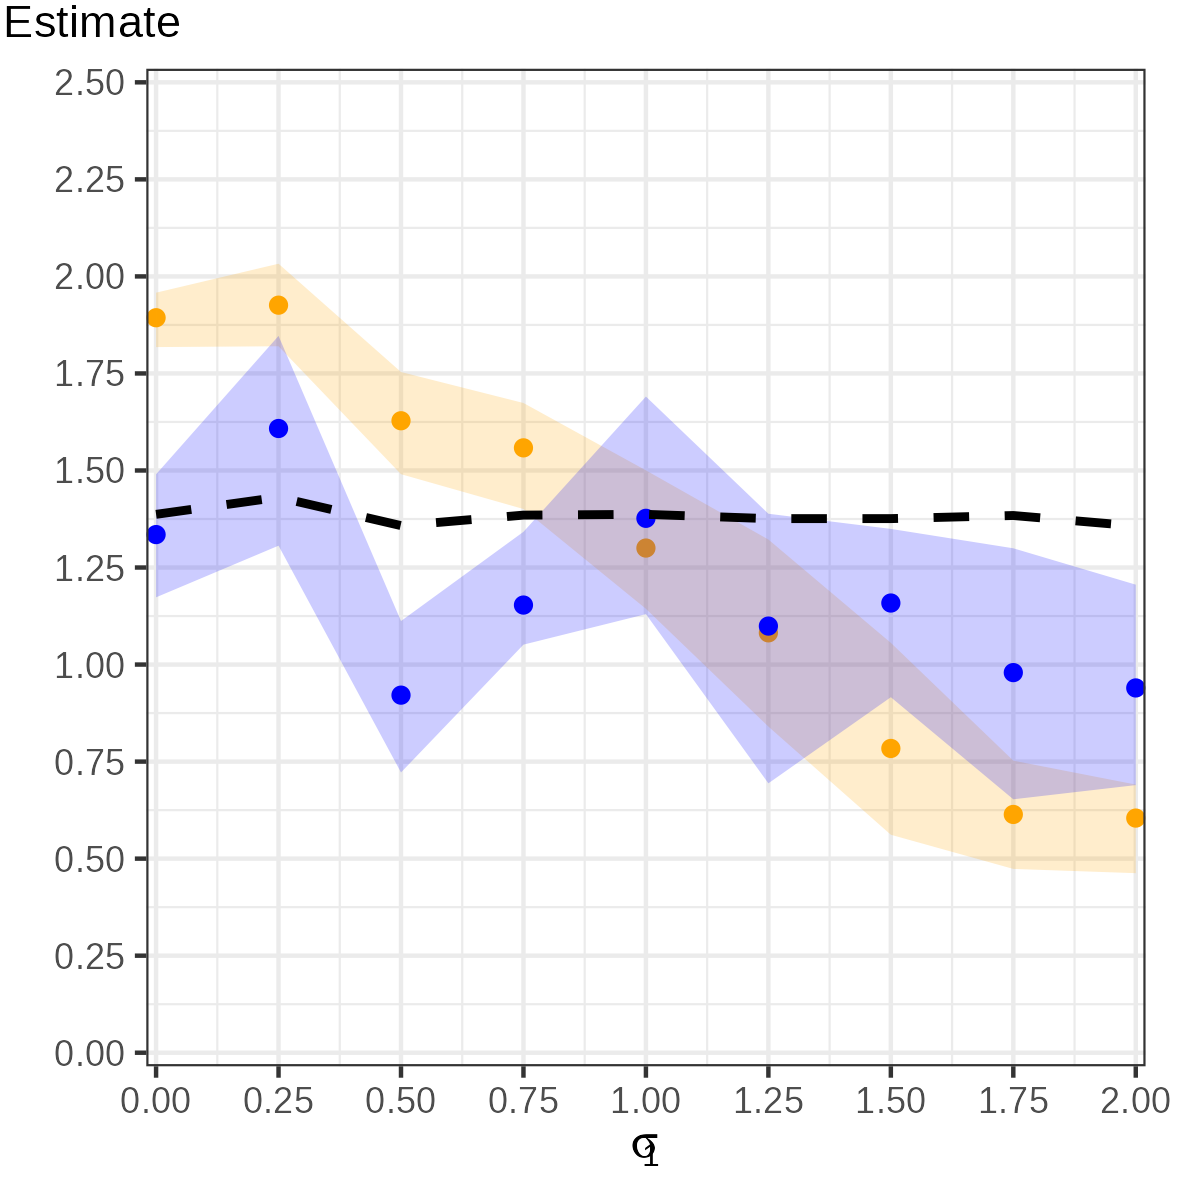
\includegraphics[width=\textwidth]{
            ../programs/simulations/sim-output/sigma1-directeffect-bias.png}
    \end{subfigure}
    \begin{subfigure}[c]{0.475\textwidth}
        \centering
        \caption{AIE.}
        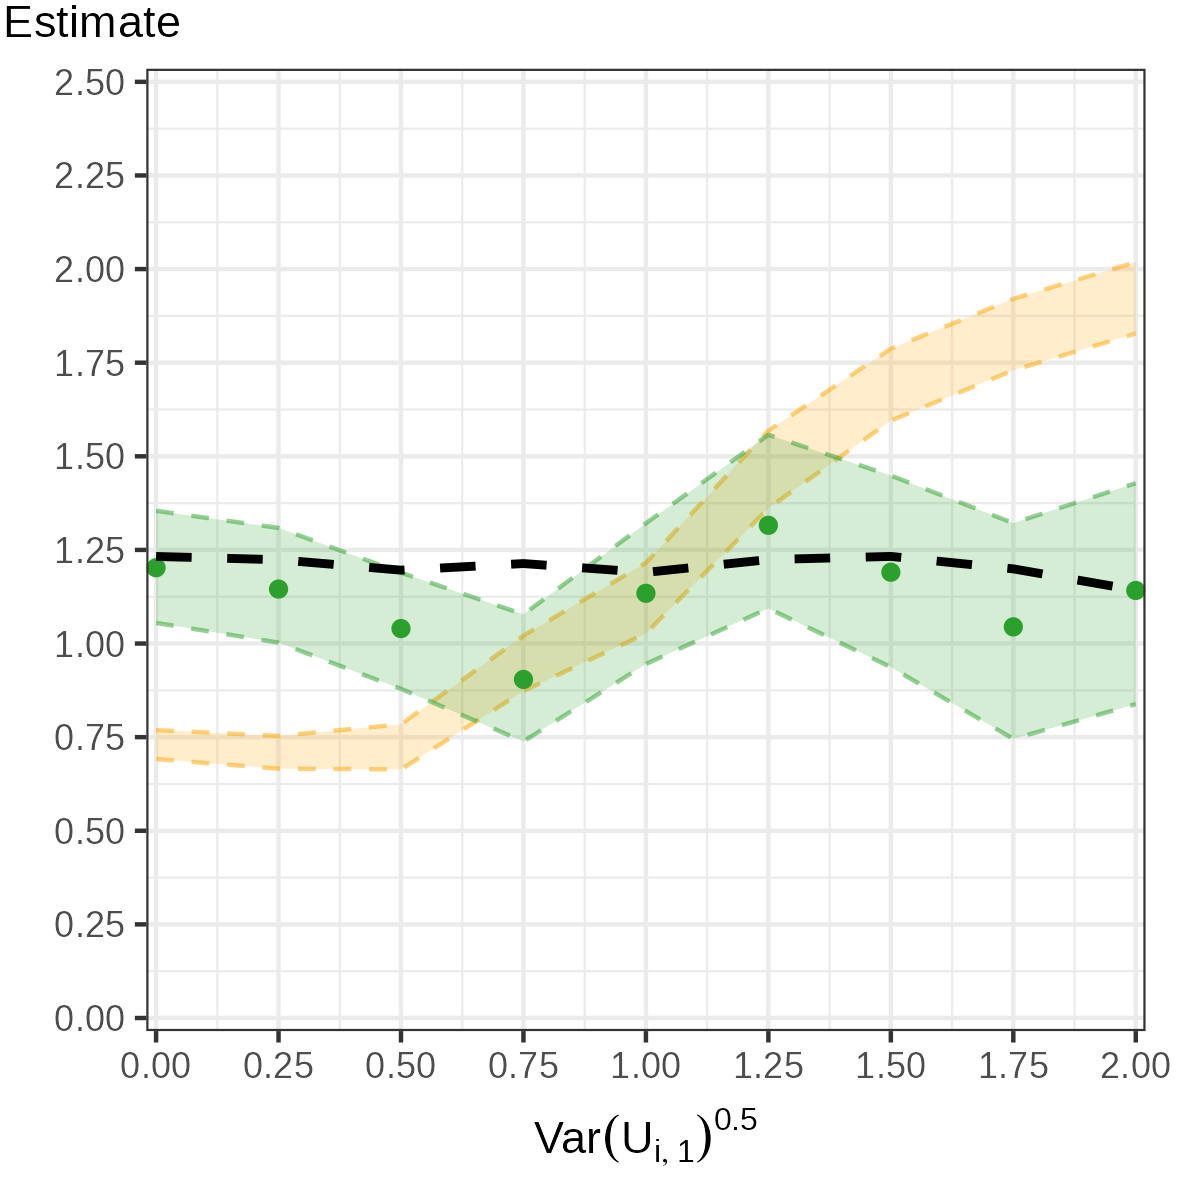
\includegraphics[width=\textwidth]{
            ../programs/simulations/sim-output/sigma1-indirecteffect-bias.png}
    \end{subfigure}
    \label{fig:sigma-1-bias}
    \justify
    \footnotesize    
    \textbf{Note:}
    These figures show the OLS and control function estimates of the ADE and AIE, for $N = 1,000$ sample size.
    The black dashed line is the true value, points are points estimates from data simulated with a given $\text{Corr}\big(U_{0,i}, U_{1,i}\big) =0.5$, $\Var{U_{0,i}} = 1$, and $\Var{U_{1,i}}^{\frac12}$ varied across $[0, 2]$.
    Shaded regions are the 95\% confidence intervals;
    orange are the OLS estimates, blue the control function approach.
\end{figure}

\end{document}
